\documentclass[english]{article}
\usepackage[utf8]{inputenc}
\usepackage[a4paper, left=3cm, right=3cm, top=4cm]{geometry}

% Language & links
\usepackage[english]{babel}
\usepackage[hidelinks]{hyperref}
\usepackage{etoolbox}

% Math
\usepackage{amsmath, amsfonts, amssymb, mathtools}
\usepackage{mathrsfs}      % script letters
\usepackage{physics}       % physics notation
\usepackage{tikz-cd}       % commutative diagrams
\usepackage{amsthm}        % proof

% Figures
\usepackage{graphicx} 
\usepackage{caption}
\usepackage{subcaption}
\usepackage[table,dvipsnames]{xcolor}
\usepackage{float}

% Tables
\usepackage{array}
\usepackage{multirow}
\usepackage{colortbl}
\usepackage{hhline}
\usepackage{booktabs}
\usepackage{booktabs}
\usepackage[table]{xcolor}

% Layout
\usepackage{tcolorbox}     % colored boxes
\usepackage{enumitem}      % custom lists
\usepackage{epigraph}      % quotes at section start
\usepackage{setspace}

% Units
\usepackage[separate-uncertainty = true]{siunitx}

% Code
\usepackage{minted}

% Appendix
\usepackage[toc]{appendix}

% Bibliography
\usepackage{csquotes}
\usepackage[backend=biber,style=numeric]{biblatex} 
\addbibresource{references.bib}

% Fix physics + siunitxW
\AtBeginDocument{\RenewCommandCopy\qty\SI}
\ExplSyntaxOn
\msg_redirect_name:nnn {siunitx}{physics-pkg}{none}
\ExplSyntaxOff

\setlength{\parindent}{0pt} % No carriage return
\onehalfspacing     % Spaziatura

\makeatletter
\def\course#1{\gdef\@course{#1}}
\def\@course{} % default value

\def\supervisor#1{\gdef\@supervisor{#1}}
\def\@supervisor{} % default value

\def\@maketitle{%
    \newpage
    \null
    \begin{center}
        % Logo
        
\includegraphics[width=0.25\linewidth]{img/logo.png}\par\vspace{1cm}
        
        % Titolo
        {\huge\scshape \@title \par}\vspace{0.5cm}
        \rule{0.7\linewidth}{0.5pt}\vspace{1cm}
    \end{center}
    
    \begin{flushright}
        {\large \@author \par}
        {\sffamily \@course \par}
        \vspace{0.5cm}
        {\Large\bfseries Supervisor: \@supervisor \par}
        \vspace{0.5cm}
        {\Large \@date \par}
    \end{flushright}
}
\makeatother

\title{Uncertainty in Financial Markets: Fractals as the Geometry of Chaos}
\author{Cerioli Gabriele, Cleva Tommaso, Daniel Chiara, Shubham Khumar, Awais Mohammad}
\supervisor{Prof. Michele Cirafici}
\date{September 2025}

\begin{document}

\maketitle

\vspace{1cm}
\begin{center}
    \epigraph{\large\textit{“I can calculate the motions of the heavenly bodies but not the madness of people”}%
    \normalsize\ }%
{\large\scshape Isaac Newton, {\ttfamily (after losing a third of his money to investments)}}
\end{center}


\vfill
\begin{center}
    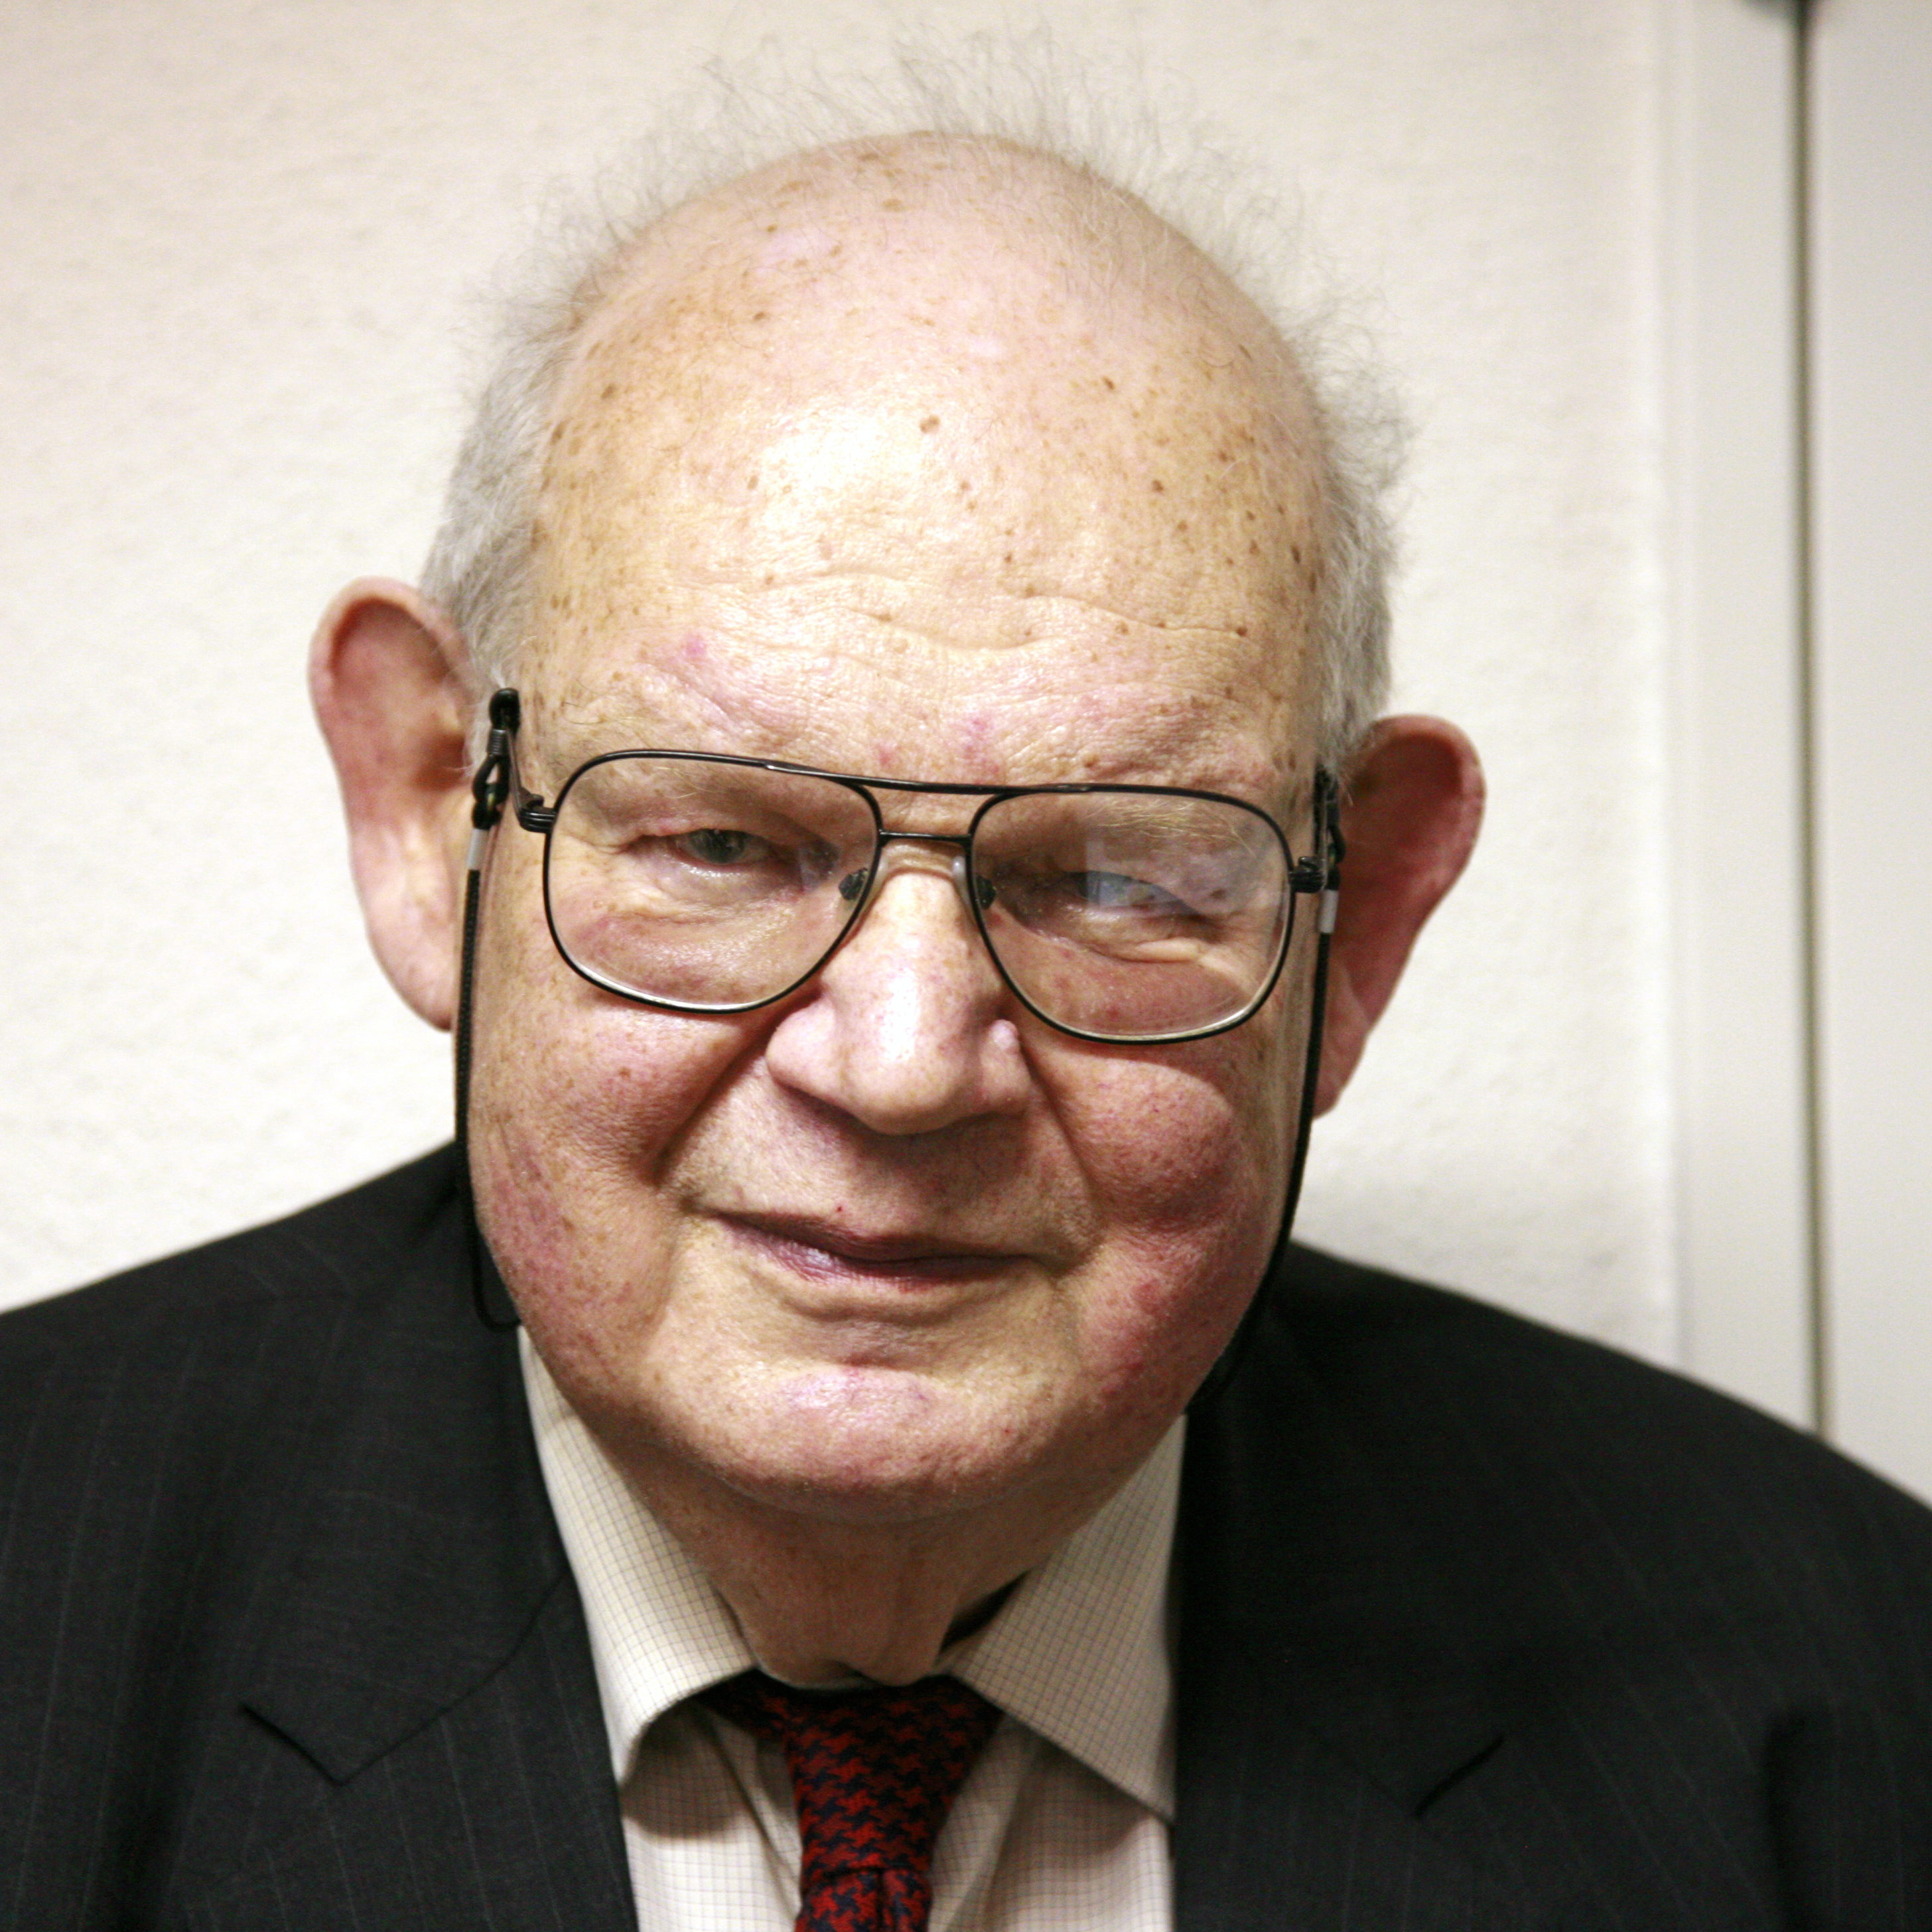
\includegraphics[width=0.5\linewidth]{img/mandelbrot.jpg}\\[0.3cm]
    \huge In memory of Professor Benoit Mandelbrot (1924--2010).\\
    %\small And in memory of Professor John Hugh Dear.
\end{center}


\newpage
\tableofcontents

\newpage
\section{Classical models for finance}
\subsection{Random walks and arithmetic brownian motion}
Imagine starting at the origin of a Cartesian plane and, every second, having the same probability of moving east, west, north, south (or even in a oblique direction). After a certain number of steps, the position you end up in is \textbf{completely unpredictable}. A \textbf{random} \textbf{walk} is a path constructed in this way, with a sequence of steps determined by probability. \\
\\
Key characteristics of a random walk:
\begin{itemize}
    \item \textbf{Unpredictable and independent increments}: Previous steps have no influence on future ones.
    \item \textbf{Variance that grows over time}: The number of possible final positions after $n$ steps increases as $n$ increases. (With a bit of reasoning, one can see that it grows proportionally to $\sqrt{n}$).
    \item \textbf{In the case of no drift}: on average, you end up at the starting point (each direction has equal probability).
\end{itemize}
We say that a random walk is driven (has a drift) when the directions have different probabilities.
%\begin{figure} [H]
%        \centering
%        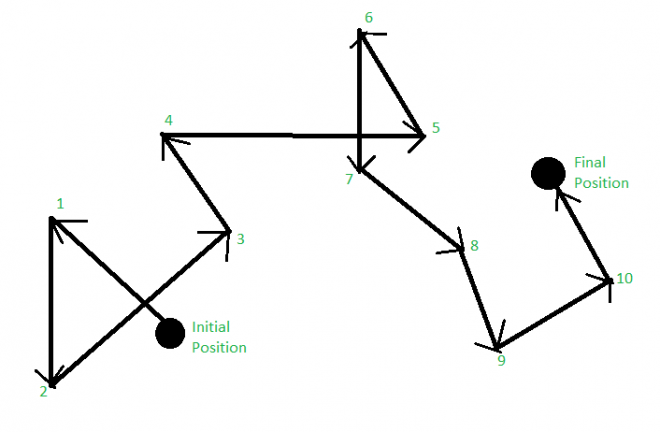
\includegraphics[width=0.5\linewidth]{img/random_walk_1.png}
%        \caption{Example of a 2D random walk}
%    \end{figure}
%\begin{figure} [H]
%    \centering
%    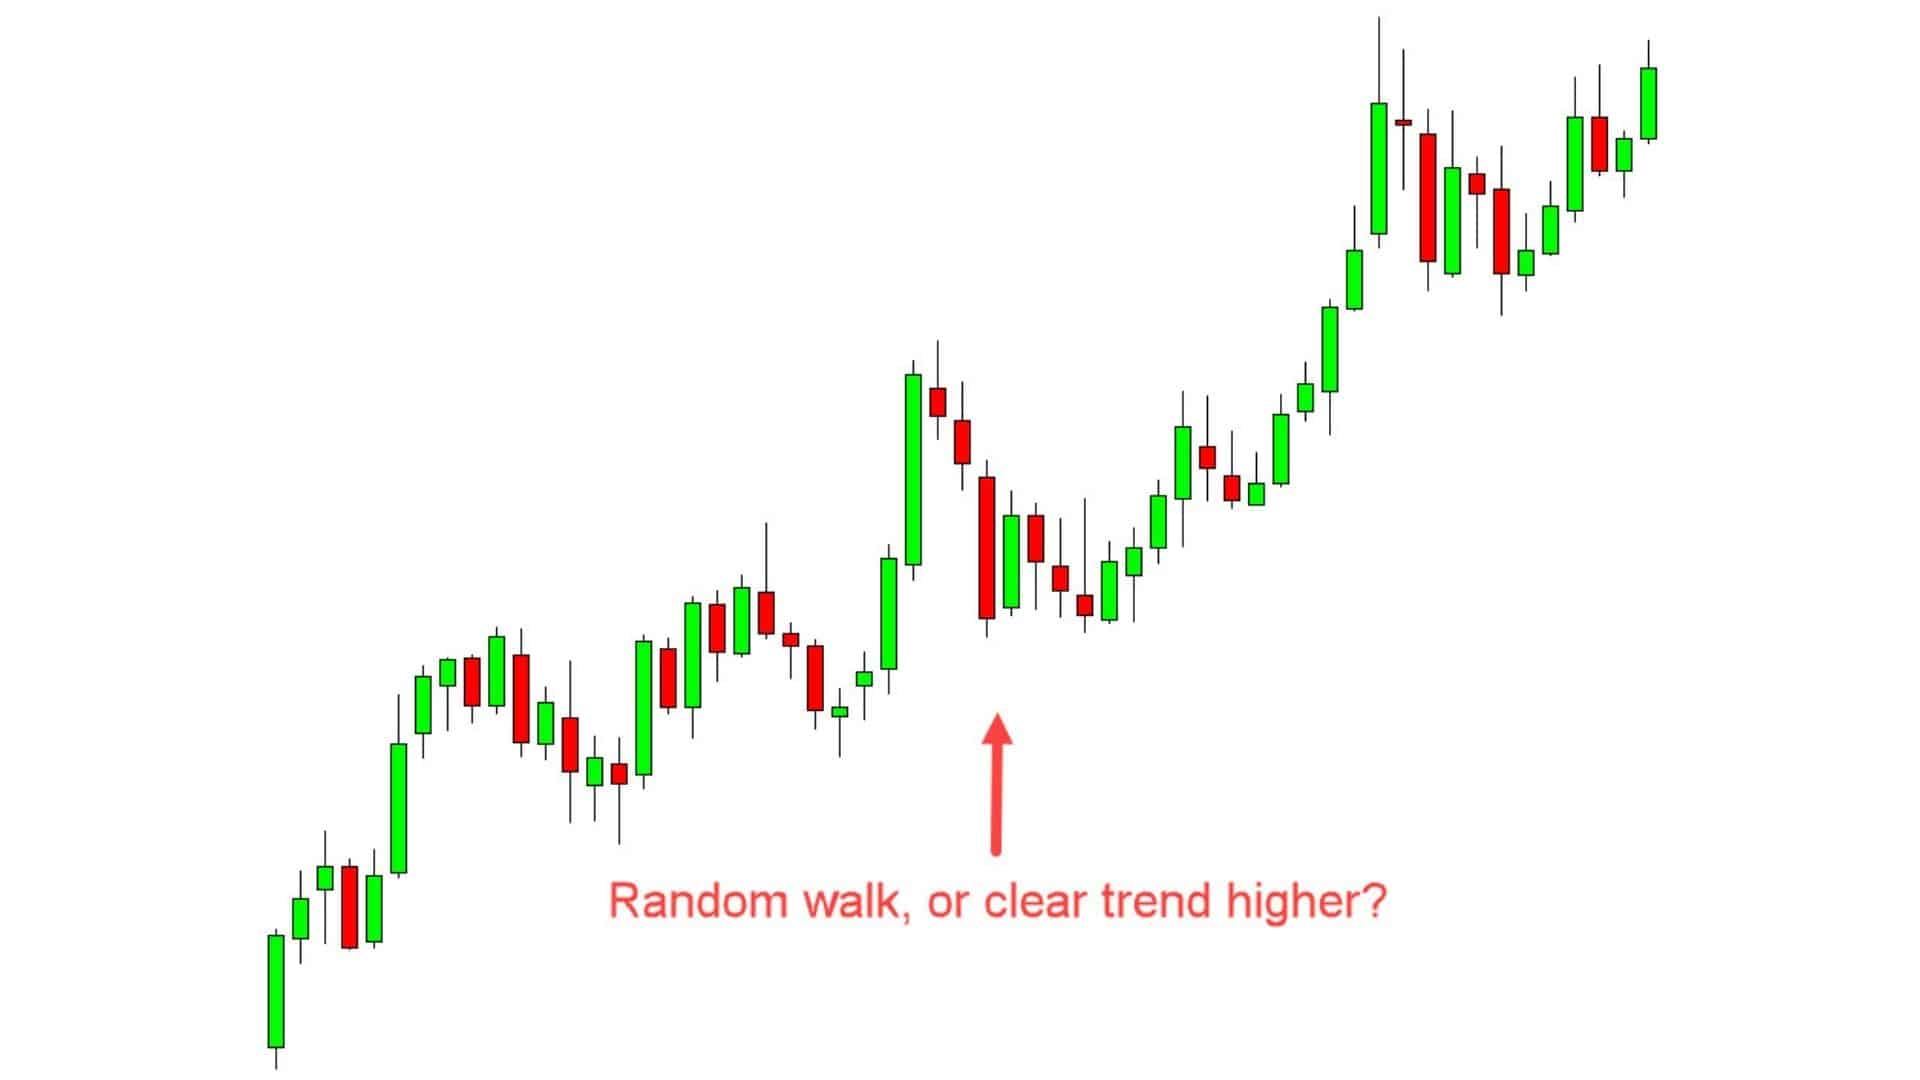
\includegraphics[width=0.75\linewidth]{img/random_walk_2.png}
%    \caption{Could one see the market as an example of a 1D random walk?}
%\end{figure}


\begin{figure}[H]
    \centering
    \begin{subfigure}{0.47\textwidth}
        \centering
        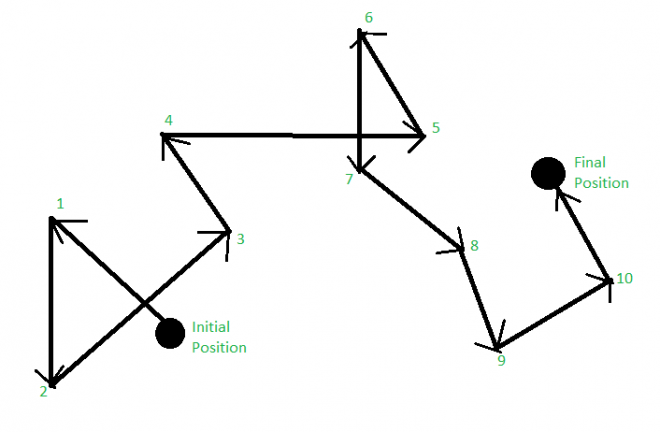
\includegraphics[width=\linewidth]{img/random_walk_1.png}
        \caption{Example of a 2D random walk.}
        \label{fig:sub1}
    \end{subfigure}
    \hfill
    \begin{subfigure}{0.47\textwidth}
        \centering
        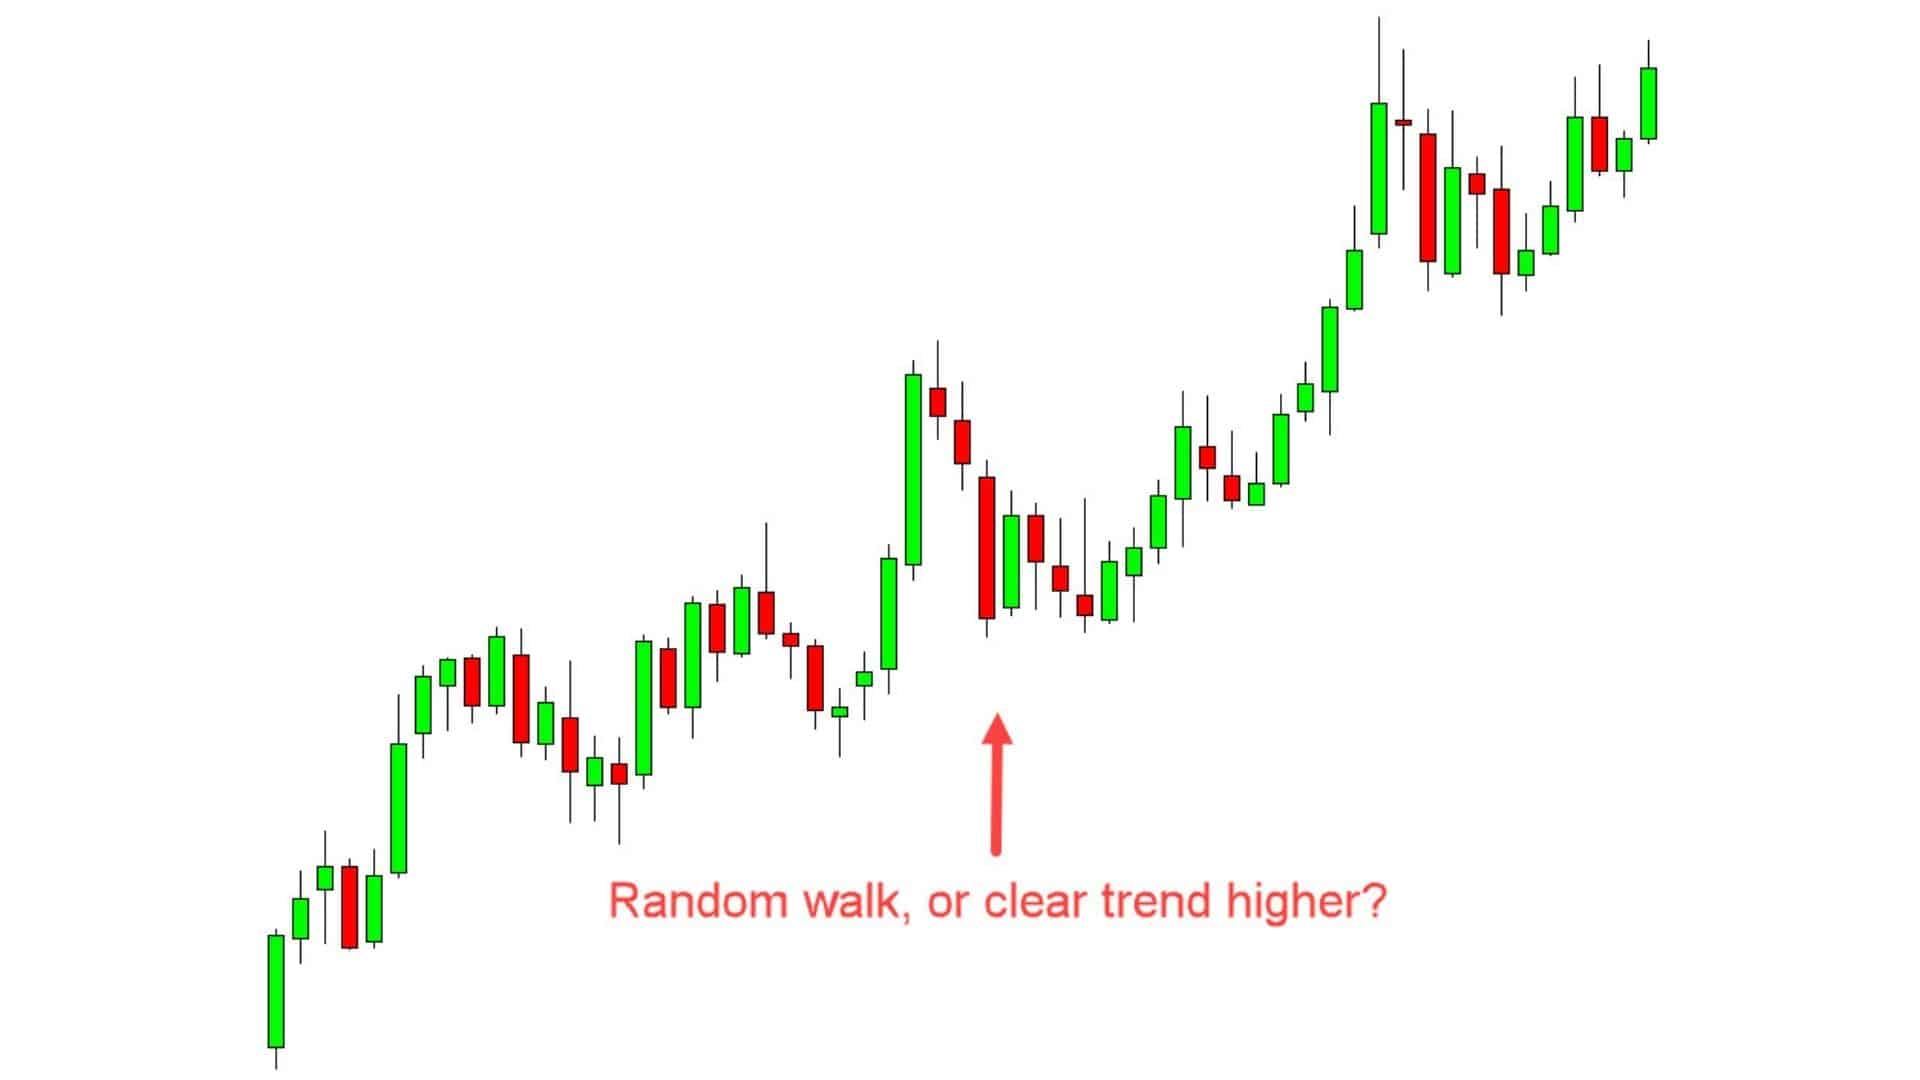
\includegraphics[width=\linewidth]{img/random_walk_2.png}
        \caption{Is the market a 1D random walk?}
        \label{fig:sub2}
    \end{subfigure}
    \caption{Examples of random walks.}
    \label{fig:due_immagini}
\end{figure}

\textbf{Arithmetic Brownian motion}: is the random motion of particles suspended in a liquid or gas medium. It consists of random fluctuations in a particle's position inside a fluid. In a fluid at thermal equilibrium there exists no preferential direction of flow (i.e. with no drift). \\
Basically the arithmetic brownian motion is a continuous-time process with Gaussian increments, essentially a continuous analogue of the random walk.\\

If you take a random walk and rescale it properly (step size $\Delta t \to 0)$ and consider jumps proportional to $\sqrt{\Delta t}$ then in the limit you obtain a Brownian motion.

\begin{figure} [H]
    \centering
    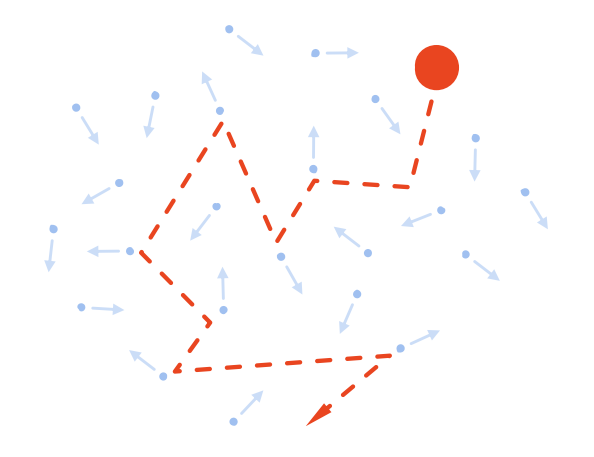
\includegraphics[width=0.5\linewidth]{img/brownian_motion.png}
    \caption{Illustration of the brownian motion of a sphere inside a fluid.}
\end{figure}

\subsection{Bachelier model}
In 1900, \textbf{Bachelier} proposed that stock prices follow a \textbf{random walk with no drift}, implying that their distribution is \textbf{normal} with a \textbf{variance proportional to time} (see Appendix \ref{app:A}).
\begin{figure} [H]
\centering
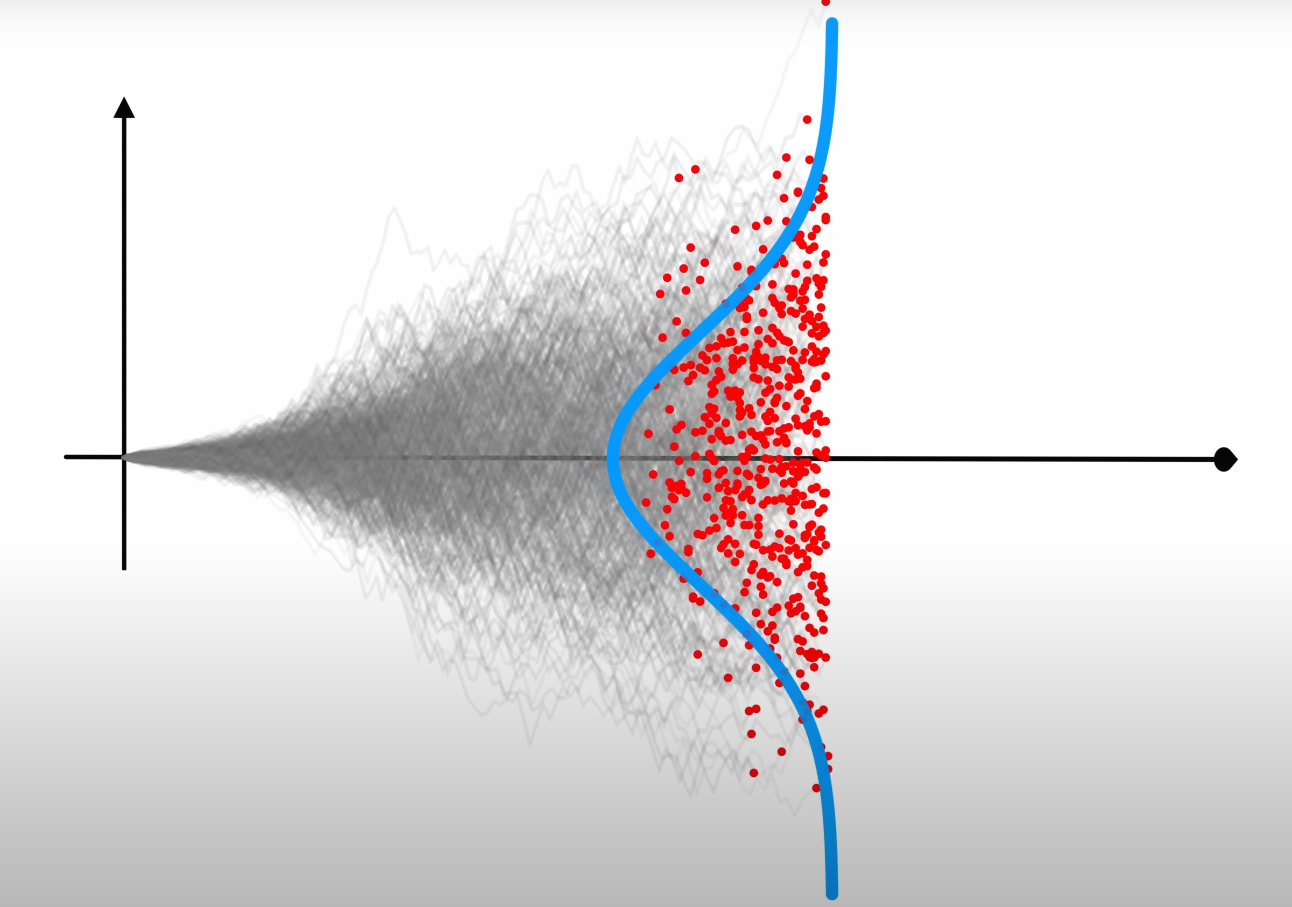
\includegraphics[width=0.5\linewidth]{img/Bachelier.png}
\caption{The stock price follows a normal distribution moving with time to the right.}
\end{figure}

An intuitive way to understand how a sequence of random walks produces a normal distribution is through the \textbf{Galton board}. In this device, balls randomly move left or right at each intersection, and the resulting pattern at the bottom naturally forms a bell-shaped curve as more balls are added.
\begin{figure} [H]
\centering
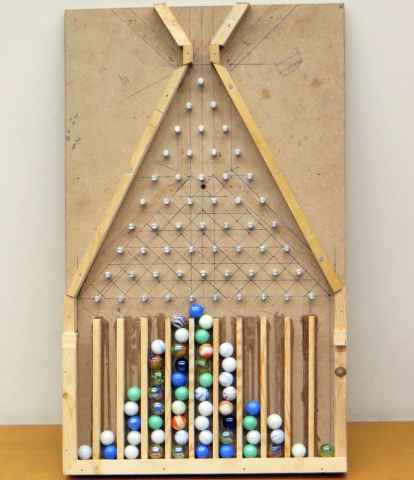
\includegraphics[width=0.5\linewidth]{img/Galton_Board_5.jpeg}
\caption{An example of Galton board.}
\end{figure}

Five years later, \textbf{Einstein} demonstrated that the same Gaussian law describes the probability distribution of particle displacements in \textbf{Brownian motion}, which is a particular solution of the \textbf{heat equation} first formulated by \textbf{Fourier} in 1822. In essence, Bachelier had anticipated that stock prices obey the same mathematical law governing the diffusion of heat from regions of high to low temperature:
\begin{equation}\label{eq:heat}
    \pdv{u}{t} = \alpha \pdv[2]{u}{x}
\end{equation} 

What we've learned to far:

\begin{table}[H]
\centering
\rowcolors{2}{gray!5}{white}
\begin{tabular}{@{}p{4cm}p{8.5cm}@{}}
\toprule
\rowcolor{gray!15}
\textbf{Model} & \textbf{Description} \\ \midrule
\textbf{Bachelier (1900)} &
Prices follow an \emph{arithmetic Brownian motion} and satisfy Fourier's heat equation. \\
\bottomrule
\end{tabular}
\caption{The Bachelier model (1900): the first stochastic model for asset prices.}
\end{table}


\subsection{The efficient Market Hypothesis (EMH)}
The \textbf{efficient-market-hypothesis} states that "\textit{asset prices reflect all available information}", basicaly you can't buy an asset and sell it immediately for profit.\\
This means that it is impossible for investors to consistently outperform the market through expert stock selection as any new information is quickly incorporated into stock prices (the more people try to predict and trade, the less predictable prices become).\\

 One can demonstrate that the EMH implies that the logarithm of stock prices follows a driven (with drift) random walk (omitted for brevity).

What we've learned so far:

\begin{table}[H]
\centering
\rowcolors{2}{gray!5}{white}
\begin{tabular}{@{}p{4cm}p{8.5cm}@{}}
\toprule
\rowcolor{gray!15}
\textbf{Model} & \textbf{Description} \\ \midrule
\textbf{Bachelier (1900)} &
Prices follow an \emph{arithmetic Brownian motion} and satisfy Fourier's heat equation. \\[3pt]
\textbf{Efficient Market Hypothesis (1960s)} &
Log-prices follow a driven random walk. \\ 
\bottomrule
\end{tabular}
\caption{From the Bachelier model to the Efficient Market Hypothesis.}
\end{table}

\subsection{Geometric Brownian Motion}

%\textbf{\large{Geometric Brownian Motion}}
\textbf{A geometric Brownian motion (GBM)} is a continuos-time stochastic process in which the logarithm of the random variable follows a Brownian motion with a drift (i.e. with a change of the average value of the random variable). \\
Using stochastic processes we can define stochastic differential equations (SDE), in which some terms and the solution are stochastic processes.
For example the SDE for the geometric brownian motion ($S_{t}$) is the following:
\begin{equation*}
    \dd S_{t} = \mu S_{t} \dd t + \sigma S_{t} \dd W_{t}
\end{equation*}
where $W_{t}$ is a Brownian motion, $\mu$ is the percentage drift and $\sigma$ is the percentage volatility.

\begin{figure} [H]
    \centering
    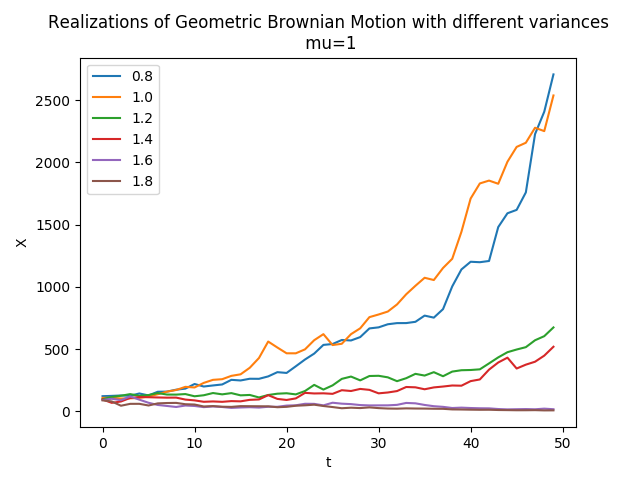
\includegraphics[width=0.75\linewidth]{img/GBM.png}
\end{figure}

\subsection{Black--Scholes--Merton Model (BSM)} 
If we take these assumptions on the market:
\begin{itemize}
    \item Ability to buy and sell any amount of the stock (without fees or costs);
    \item Ability to borrow and lend any amount at the riskless rate (without fees or costs);
    \end{itemize}
    and if it follows the efficient market hypothesis:
    \begin{itemize}
    \item There is a \textbf{risk-free interest rate} and it is \textbf{constant}. There is \textbf{no arbitrage} opportunity (there is no way to make a riskless profit exceeding the risk-free rate);
    \item The stock does not pay a dividend.
    \end{itemize}
Then not only the log return of the stock price follows a driven random walk (EMH), but the stock price follows a Geometric brownian motion:
\begin{equation*}
    \dd S = S \dd t + \sigma S \dd z
\end{equation*}
where $\dd S$ is the infinitesimale change in stock price, $S \dd t$ is the drift, and $\sigma S \dd z$ is randomness term, basically a brownian motion with drift.\\

After some number of steps, one should get the Black--Scholes/Merton equation:
\begin{equation} \label{eq:Black–Scholes}
    \pdv{V}{t} + rS \pdv{V}{S} + \frac{1}{2} \sigma^2 S^2 \pdv[2]{V}{S} - rV = 0
\end{equation}
In this case, since the log of the price follows an arithmetic brownian motion, it also solves the Fourier's heat equation.
We refer to Appendix~\ref{app:B} for the derivation transforming the Black--Scholes equation into the heat equation, and to Appendix~\ref{app:B_solution_Black-Scholes} for the detailed calculations leading to its solution.

What we've learned so far:

\begin{table}[H]
\centering
\rowcolors{2}{gray!5}{white}
\begin{tabular}{@{}p{3.8cm}p{8.2cm}@{}}
\toprule
\rowcolor{gray!15}
\textbf{Model} & \textbf{Description} \\ \midrule
\textbf{Bachelier (1900)} &
Prices follow an \emph{arithmetic Brownian motion} and satisfy Fourier's heat equation. \\[2pt]
\textbf{Efficient Market Hypothesis (1960s)} &
Log-prices follow a driven random walk. \\[2pt]
\textbf{Black–Scholes / Merton (1970s)} &
Prices follow a \emph{geometric Brownian motion}, hence log-prices satisfy Fourier's heat equation. \\ 
\bottomrule
\end{tabular}
\caption{From Bachelier to Black–Scholes: evolution of price modeling.}
\end{table}



\section{Black Swans in the stock puddle}

\begin{figure}[H]
    \centering
    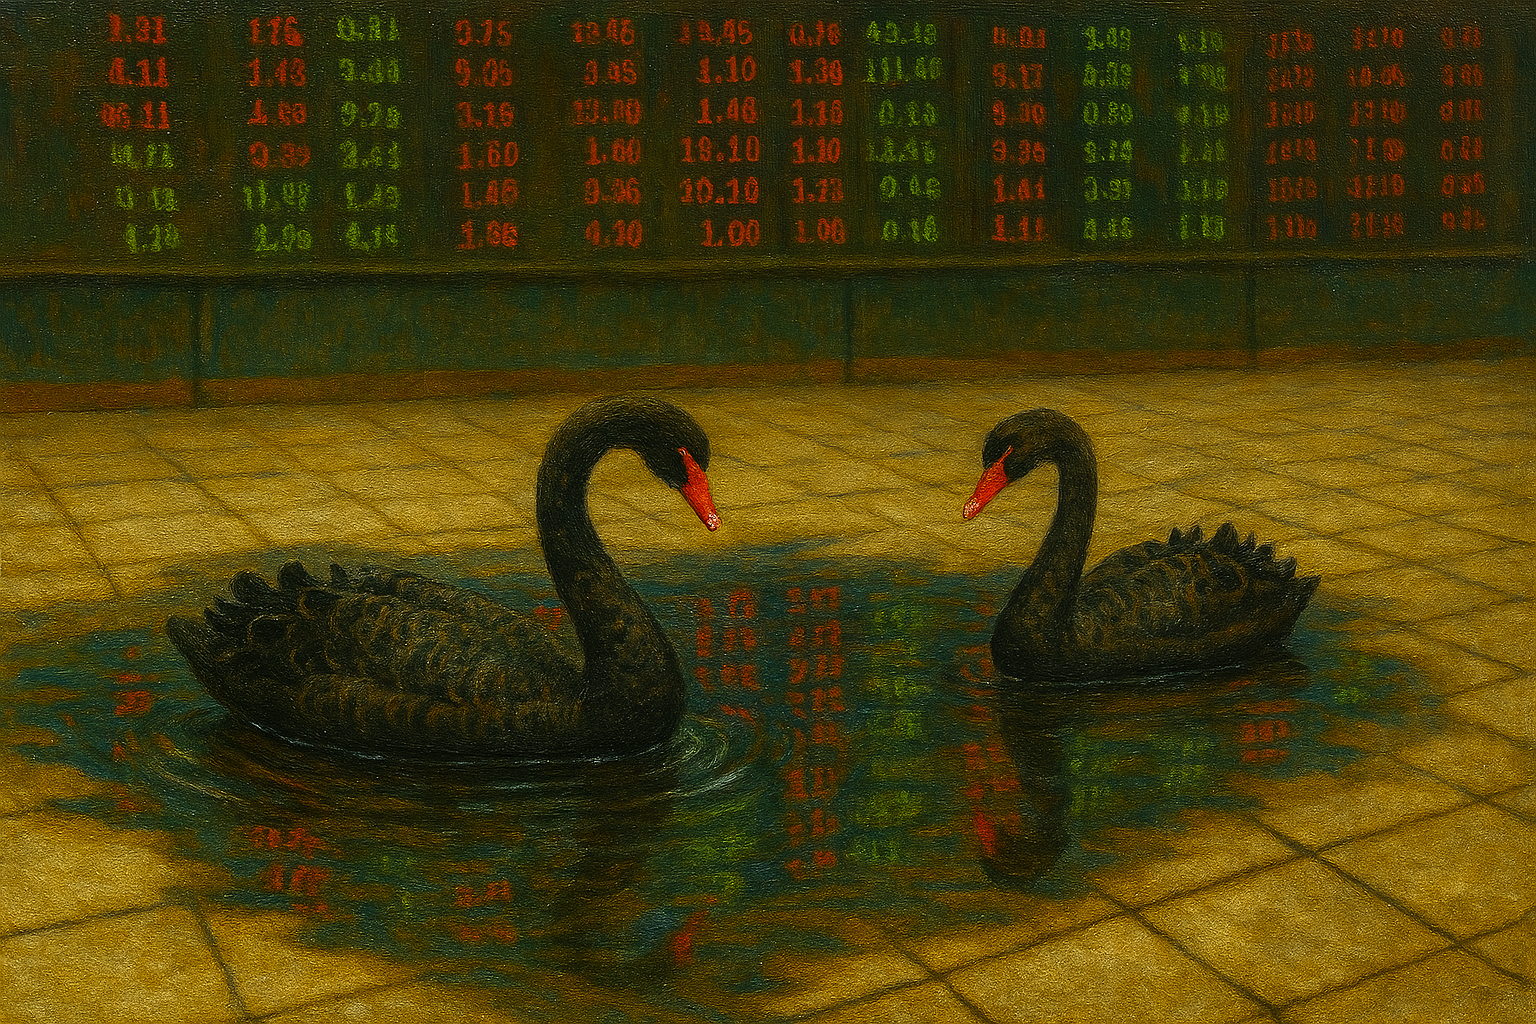
\includegraphics[width=0.65\linewidth]{img/Copilot_20250925_235000.png}
\end{figure}
\textit{A black swan is an event in the stock market that exceeds six standard deviations, an "almost" impossible event. }
\begin{itemize}
    \item On October 19, 1987 (Black Monday), the Dow Jones Industrial Average fell 29.2 percent, based on classical theories the probability of such an event was less than one in $10^{50}$ odds. This is a number outside the scale of nature, it is like tossing 166 coins and getting 166 heads. Imagine choosing one specific molecule of water from all the oceans on Earth — that’s roughly a 1 in $10^{46}$ chance. Now make it 10000 times rarer.
\end{itemize}
It surely had been an event of extremely bad luck, a freak accident, an unpredictable "act of God", or was it?
\begin{itemize}

\item In the summer of 1998 the improbable happened: on August 4 the Dow index fell 3.5$\%$, three weeks later by 4.4$\%$ and then again on August 31 by 6.8$\%$. This should never have happened, about one in 500 billion chance. You should not expect to see something like this even if you traded for 2.5 million years.
\item A year earlier (1997), the Dow had fallen 7.7$\%$ in one day with a probability of one in 50 billion.
\item In July 2002, the index recorded three steep falls within seven trading days, (one in four trillion).
\end{itemize}
\textbf{The reader should already have grasped--without the need to list more of the many such events—that there is something fundamentally flawed in the way the probability of these rare events is assessed.}

\section{Why fractals: modeling uncertainty through fractal analysis}
\subsection{Power laws and fat tails distributions}
Examine price records more closely, and you typically find a different kind of distribution than the bell curve: the tails follow a "\textbf{power law}". These are common in nature: if the sizes of the sides of a square doubles, the area quadruples, if the side triples, the area rises nine-fold; gravity weakens by the inverse power of two with the distance, ...\\

In 1962 Benoit Mandelbrot showed that positive and negative price movements follow power laws rather than normal distributions.
\begin{figure} [H]
    \centering
    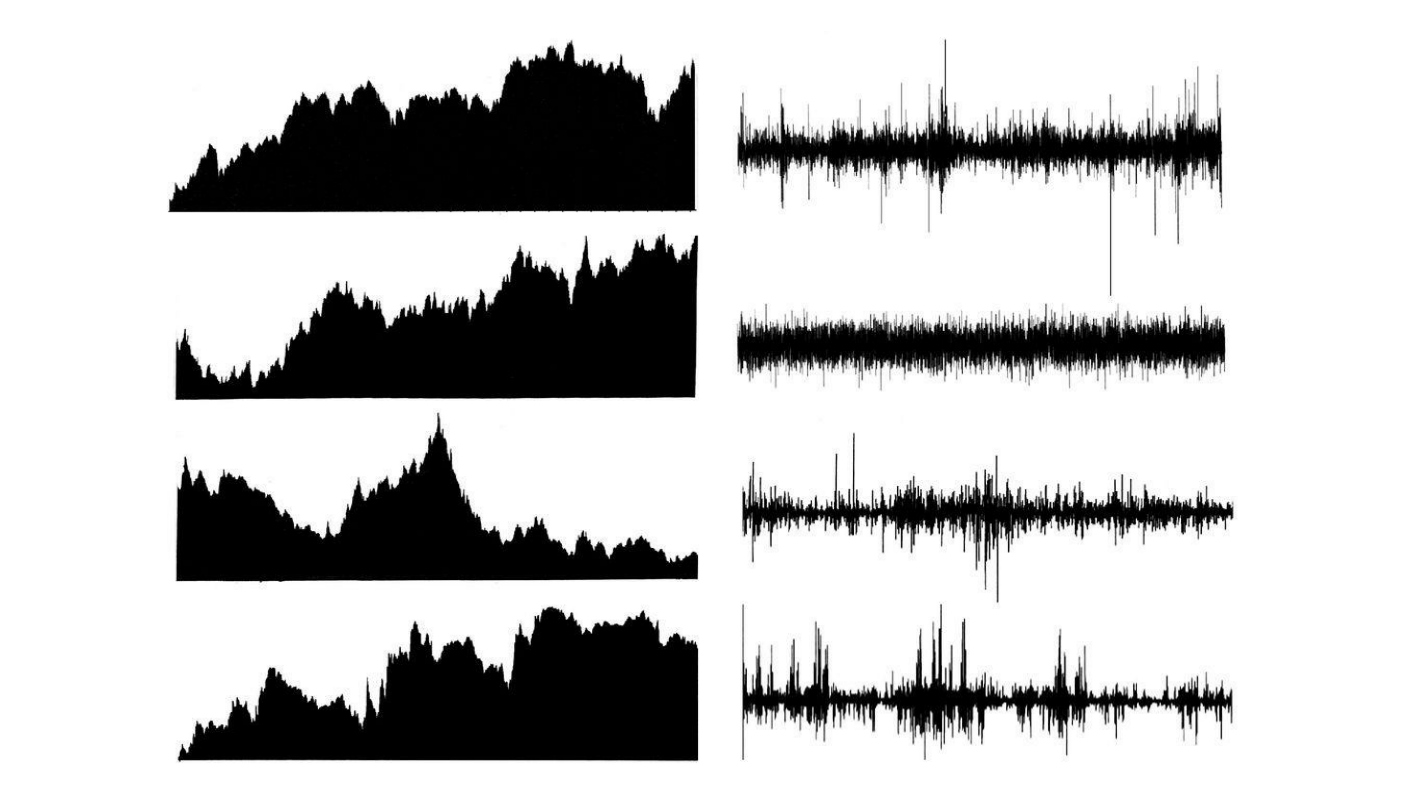
\includegraphics[width=1\linewidth]{img/market_comparison.jpg}
    \caption{On the left there are 4 price charts, the first and third are real chronicles, the second one is generated using classical models (BSM) and the last one is generated with one of the latest fractal and fat tails model. They pretty much look the same. To discover the differences one should look at the graph of the changes in logprice from moment to moment (shown on the left).}
    %\label{fig:placeholder}
\end{figure}
Power laws can be distributions with fat tails, meaning that the tail (the extreme values, the ones far from the mean) drops off more slowly than a thin tail (for example in the normal distribution).

An event 8 standard deviation from the mean:
\begin{itemize}
    \item In a normal distribution, it has a probability of $6 \cross 10^{-16}$;
    \item In a power law distribution, it can have a probability of almost $4 \%$, much higher.
\end{itemize}

Using a thin-tailed model for a fat-tailed phenomenon means underestimating risk of extreme events.
\begin{figure} [H]
    \centering
    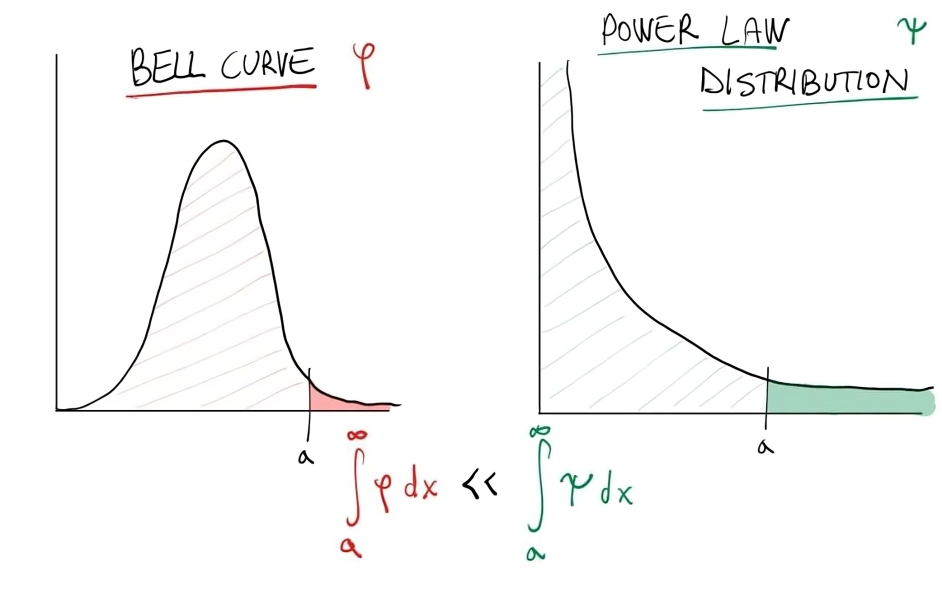
\includegraphics[width=0.65\linewidth]{img/WhatsApp Image 2025-10-04 at 22.22.36.png}
    \caption{Normal distribution vs Power law Distribution.}
    %\label{fig:placeholder}
\end{figure}

\subsection{What are fractals?}
"\textit{A fractal is a rough or fragmented geometric shape that can be split into parts, each of which is (at least approximately) a reduced-size copy of the whole}" (Benoit Mandelbrot). \\

Among the features of a fractal we can find:
\begin{itemize}
    \item Self-similarity;
    \item Fine or detailed structure at arbitrarily small scales;
    \item Irregularity both locally and globally, that cannot easily be described with traditional Euclidean geometry without the use of recursion.
\end{itemize}
For example, a straight line is not a fractal, since it is self similar but it lacks detail and can be described with Euclidean geometry without the need for recursion.
\begin{figure} [H]
    \centering
    
\includegraphics[width=0.65\linewidth]{img/Mandel_zoom_00_mandelbrot_set.jpg}
    \caption{The boundary of the Mandelbrot set is a fractal curve.}
\end{figure}
\subsection{Fractality in the financial market}
\textbf{What evidence suggests that financial markets may exhibit fractal properties?}
\begin{itemize}
    \item When comparing the price charts and log-returns of different financial markets, it is very difficult to identify significant differences.
    \begin{figure} [H]
        \centering
        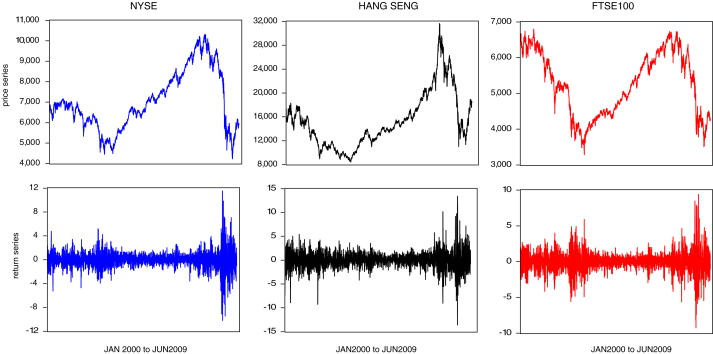
\includegraphics[width=1\linewidth]{img/fractal_1.png}
        \caption{There are very little differences in these three different financial markets.}
    \end{figure}
    \item If we take the liberty of examining the price charts of the New York Stock Exchange (NYSE) while concealing the axis labels and applying suitable dilations or contractions along the vertical axis, it becomes impossible to distinguish one time scale from another—that is, whether we are observing price variations over the course of a single day or an entire year.

\begin{figure}[htbp]
    \centering
    % --- Prima riga ---
    \begin{subfigure}{0.45\textwidth}
        \centering
        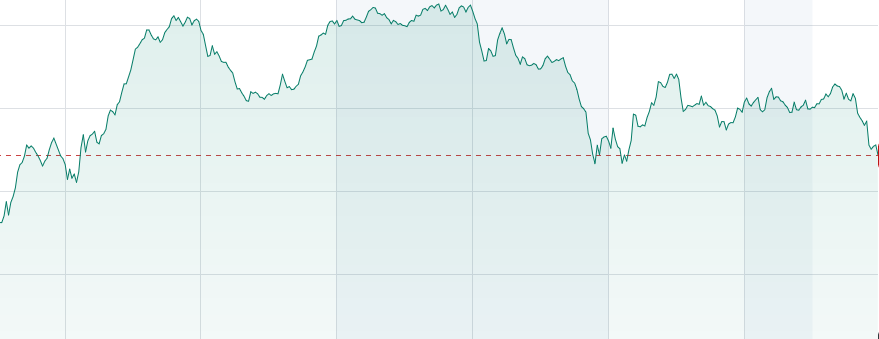
\includegraphics[width=\linewidth]{img/1d.png}
        \caption{Price over 1 day.}
    \end{subfigure}
    \hfill
    \begin{subfigure}{0.45\textwidth}
        \centering
        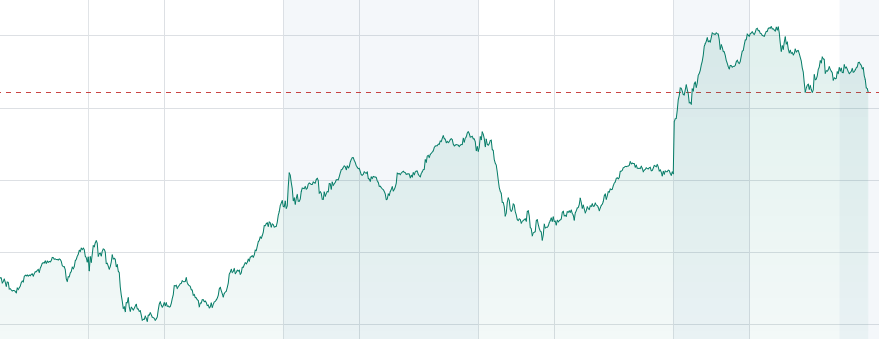
\includegraphics[width=\linewidth]{img/5d.png}
        \caption{Price over 5 days.}
    \end{subfigure}

    % --- Seconda riga ---
    \begin{subfigure}{0.45\textwidth}
        \centering
        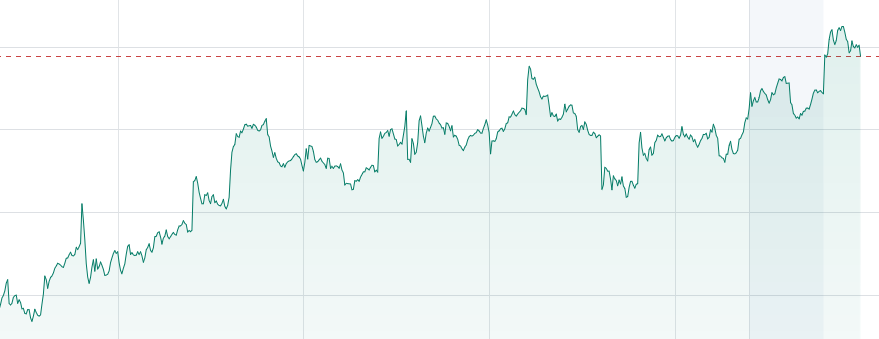
\includegraphics[width=\linewidth]{img/1m.png}
        \caption{Price over 1 month.}
    \end{subfigure}
    \hfill
    \begin{subfigure}{0.45\textwidth}
        \centering
        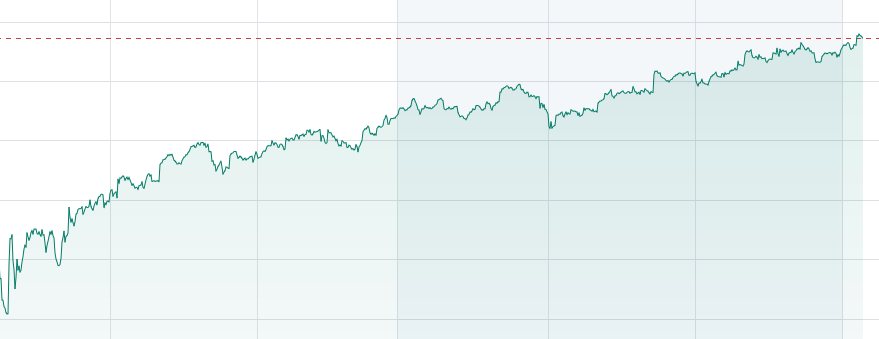
\includegraphics[width=\linewidth]{img/1y.png}
        \caption{Price over 1 year.}
    \end{subfigure}

    % --- Terza riga ---
    \begin{subfigure}{0.45\textwidth}
        \centering
        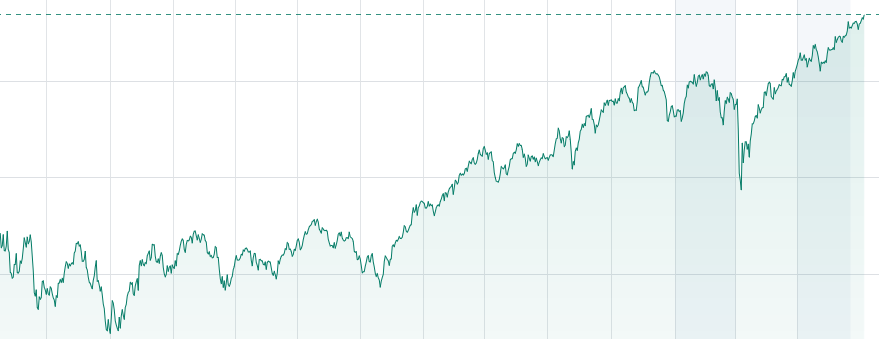
\includegraphics[width=\linewidth]{img/5y.png}
        \caption{Price over 5 years.}
    \end{subfigure}
    \hfill
    \begin{subfigure}{0.45\textwidth}
        \centering
        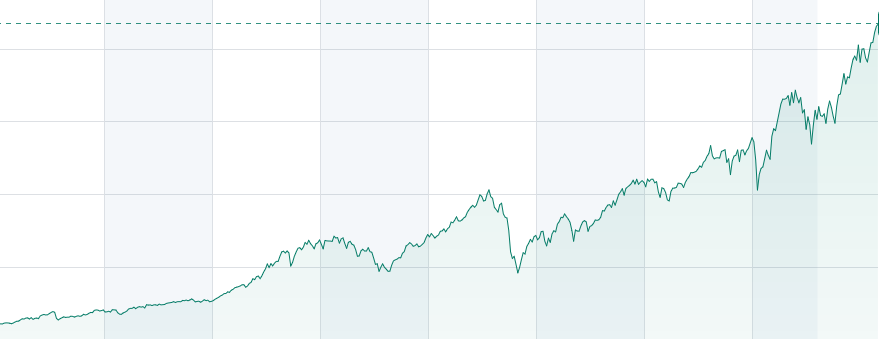
\includegraphics[width=\linewidth]{img/30y.png}
        \caption{Price over 30 years.}
    \end{subfigure}
        \caption{Prices of NYSE Composite Index at different time scales.}
    \label{fig:siximages}
\end{figure}
    It is evident from the simple experiment just carried out that financial markets exhibit \textbf{self~-~similarity} across different time scales and detailed structure at arbitrarily small scales.
\end{itemize}

\subsection{Chaos in the financial market}
Another characteristic that helps explain the irregularity of financial markets is their \textbf{chaotic nature}. Sudden crashes, bursts of volatility, and persistent cycles suggest that markets may not be purely random, but rather governed by nonlinear dynamics that resemble chaotic systems.\\

Chaos does not imply complete disorder. Instead, it refers to systems that are deterministic in structure yet highly sensitive to initial conditions a phenomenon widely known as the “Butterfly Effect.” This sensitivity makes long-term prediction practically impossible, even when the underlying rules are well defined.\\

As we will illustrate with an example in this chapter, the chaotic nature of financial dynamics can be detected in real BTC-USD price data.\\
In particular, we will find that the data follow an \textbf{attractor}, that is, a set of states toward which the system tends to evolve over time, regardless of small modifications to the initial conditions. Specifically, the attractor we will identify is a \textbf{strange attractor}, a hallmark of a chaotic system, since its fractal dimension is non-integer, thereby exhibiting self-similarity across different scales and trajectories that never repeat exactly, while still remaining within the basin of attraction.
\begin{figure} [H]
    \centering
    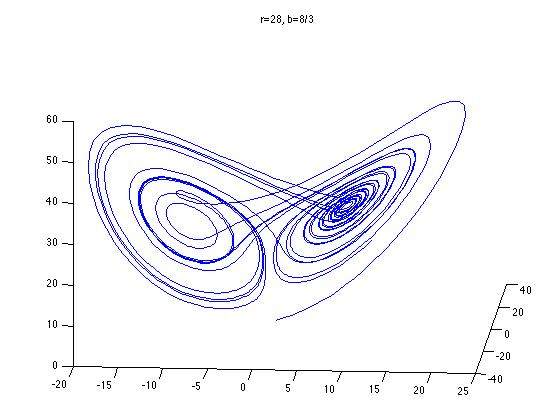
\includegraphics[width=0.75\linewidth]{img/image.png}
    \caption{A Lorentz attractor, a very well known example of strange attractor.}
\end{figure}

\subsection{Takens' Theorem: The importance of the Past in Reconstructing the future}
Having introduced the notion of strange attractors as the geometric signature of chaos, we are now in a position to ask how such structures can be uncovered from real data.\\

In practice, we rarely have access to the full set of equations governing a system; instead, we typically observe only a \textbf{single time series}, such as a financial price.\\

\textbf{Takens' embedding theorem} (1981, Floris Takens) represents a cornerstone in the study of nonlinear dynamics and chaos.\\

At its core, the theorem demonstrates that it is possible to reconstruct the underlying structure of a dynamical system (even if it shows chaotic behavior) by observing only a single time series of measurements.\\

This justifies the use of \textbf{time-delay embedding methods} to forecast the behavior of chaotic systems such as financial markets. An example of these methods will be discussed in the following chapter.\\

A mathematically rigorous formulation of the theorem's statement would require advanced knowledge and would certainly fall beyond the scope of this review.\\

Nevertheless we can still grasp the general idea of the theorem, but since it is not essential for understanding the following chapters, what follows may be skipped:\\

\textit{Suppose we have a $d$-dimensional state vector $x_t$ that evolves according to an unkown but continuous and deterministic dynamic.} \textit{In simple terms, we require that the differential equations governing the system be continuous and deterministic. This is crucial, since if the system were purely stochastic, there would be no way to reconstruct its evolution.}\\
\textit{Suppose, too, that the one-dimensional observable $y$ is a smooth function of $x$, and coupled to all the components of $x$. In our case this $y$ may be the price at a given time.}\\

\textit{At any time we can look not just at the present measurement $y(t)$, but also at observations made at times removed from us by multiples of some lag $\tau$: $y_{t+\tau},y_{t+2\tau},...$.\\}
\textit{If we use $k$ lags, we will have a $k$-dimensional vector.\\}
\textit{As one might expect, in the limit $k \to \infty$ the motion on the lagged space becomes deterministic at a finite dimension; not only that, but this deterministic dynamics (in the lagged space) are equivalent to those of the original state space. (They are related by a smooth, invertible change of coordinates, or if you like it more a diffeomorphism.)}



\subsection{How fractals can explain the market? (k-NN method)}\label{sec:k-NN_method}
Many algorithms use fractals in an attempt to forecast market prices, let us now explore one of the most widely used algorithms, called the k-NN method (k-nearest neighbours), which exploits fractal dimension and lag points to account for the irregularities in past data, as justified by Takens's theorem.
\begin{itemize}
    \item \textbf{Make a lag plot of your price data}:\\
    Consider the price series $\{x_i,i=1,...,n\}$, to build a lag plot, you take this time series and plot each value against its lagged version. For example, if you choose a lag of 1, you plot the pairs $(x_i,x_{i-1})$.\\
The horizontal axis represents the lagged values, while the vertical axis represents the current values. By varying the lag length ($L$), you can explore how the present depends on past observations. If the points appear randomly scattered, the series has little temporal dependence; if patterns or structures emerge, this indicates correlations or nonlinear dynamics in the data.
    \item \textbf{Compute the fractal dimension:}\\
    Now we need to compute the fractal dimension of the time series in order to measure how the complexity of the data changes with scale. \\
    You can compute the fractal dimension with the \textbf{box-counting method}: \\

    Cover the whole set of points with $\varepsilon$-sized boxes (in our case you need to cover the points in the lag-plot with squares, 2-D boxes).\\
    Then count the number of boxes you used $N(\varepsilon)$ and take the limit $\varepsilon \to 0$ to get the box-dimension:
    \begin{equation*}
         f=\lim_{\varepsilon \rightarrow 0} \frac{\ln(N(\varepsilon))}{\ln(1/\varepsilon)}    
    \end{equation*}
    
    There are plenty of other algorithms that one may use to compute the fractal dimension of a set of points (as the correlation dimension explained in Appendix \ref{app:C_Correlation_dimension}).
    \item \textbf{Find the optimal lag length} $\boldsymbol{\tilde{L}}$:\\
    It is necessary to decide the length of the lag. If it is too short, the reconstructed space does not capture enough of the underlying structure; if it is too long, the representation becomes redundant and noisy.\\
    
    
    The lag length specifies the number of steps back in time that must be considered when constructing the pairs in the lag plot. \\
    For example if you have a lag length of $L=2$ the pairs of the lag plot are $(x_t,x_{t-2})$ \textit{(there's a generalisation to a multilag embedding that consider all the $L$ previous lagged values. So in the previous case the lag plot will be a 3-D plot with points $(x_t,x_{t-1},x_{t-2})$, and so on for higher values of $L$)}.\\

    
    A practical way to determine the optimal lag length ($\tilde{L}$) is to compute the fractal dimension of the lag plots for increasing lag values.\\
    You expect to see something like this:
    \begin{figure}[H]
        \centering
        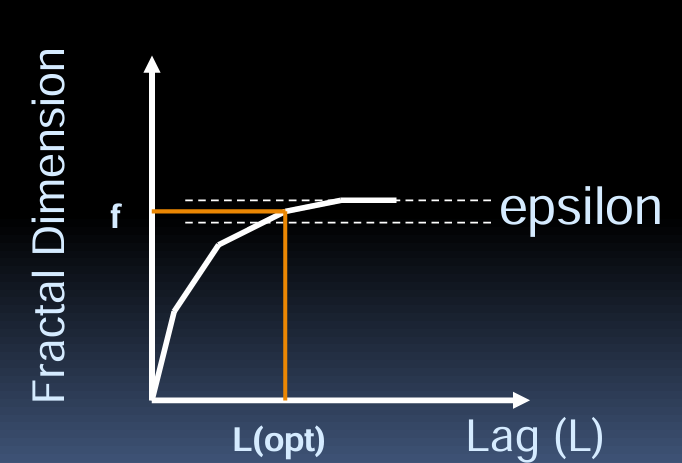
\includegraphics[width=0.6\linewidth]{img/image2.png}
        \caption{Fractal dimension of the lag plots for increasing lag values.}
        %\label{fig:placeholder}
    \end{figure}
    As the lag grows, the estimated fractal dimension will initially increase, since we are discovering new independent information. At some point, however, the dimension stabilizes within a fixed small tolerance ($\varepsilon$). The lag value at which this stabilization occurs is chosen as the optimal lag length $\tilde{L}$.\\

    
    (\textit{In the multi-lag embedding you can compute the fractal dimension by covering the $N$-dimensional plot with hyper-cubes})\\

    
    Basically what we have computed is the smallest number of past observations needed to capture the intrinsic complexity of the time series without adding unnecessary redundancy.
    \item \textbf{Optimal number of lag points:}\\
    The aim here is doing an interpolation within a set of nearest neighbors of the current point.\\
    But we need to choose the optimal number of neighbouring lag points $\tilde{k}$.\\
    If too few neighbors are selected, the interpolation becomes unstable and overly sensitive to noise: however if too many are included, the prediction is oversmoothed and loses the local structure of the dynamics. \\

    
    There's a conjecture proposing that the optimal number of neighbors is directly related to the fractal dimension $(f)$:
    \begin{equation*}
        \tilde{k} \sim  \mathcal{O}(f)
    \end{equation*}
    and more specifically, a practical rule of thumb is given by: $\tilde{k}=2f+1$.


    The conjecture is of course meaningful:
    \begin{itemize}
        \item An higher fractal dimension $f$ indicates more irregularity whose local geometry  can only be captured with more neighbors;
        \item Conversely, a lower $f$ corresponds to smoother dynamics, where fewer neighbors are sufficient.
    \end{itemize}
    \item \textbf{Nearest Neighbours Interpolation:}\\
    We perform interpolation using the nearest neighbours, since we believe that similar past states tend to evolve in similar ways. 
    We need to reconstruct the lag plot (using $\tilde{L}$) and choose a distance metric (typically the Euclidean distance) to identify the $\tilde{k}$ nearest neighbours.

    Once the nearest neighbours are identified, their subsequent values (what their values have become) are collected and used to estimate the future of the current state.\\
    \\
\begin{figure} [H]
    \centering
    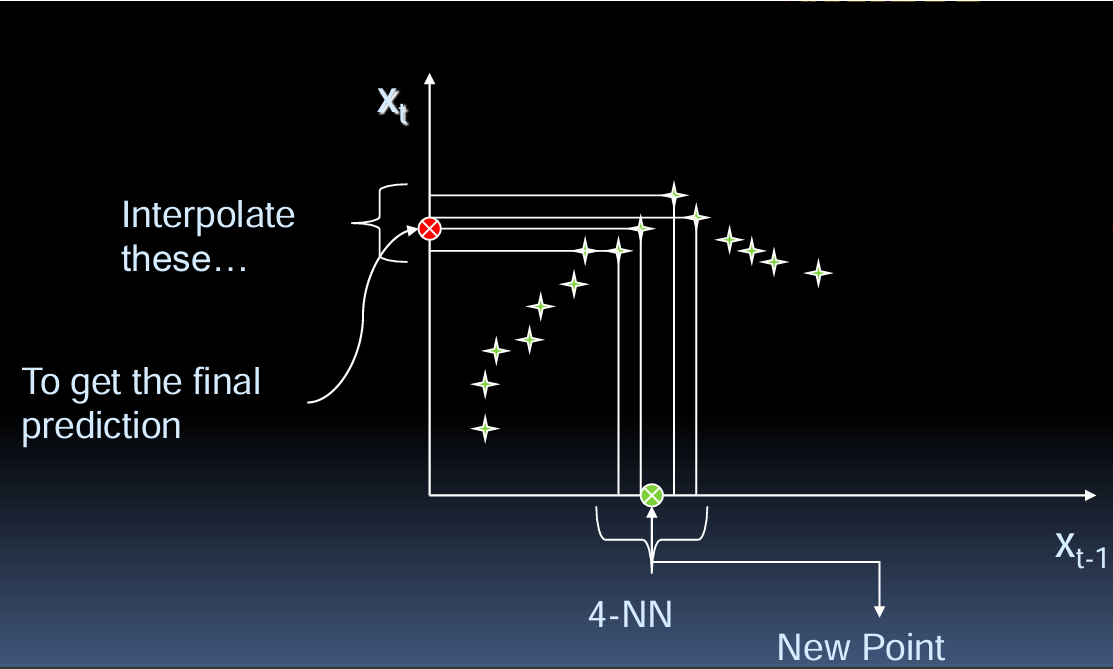
\includegraphics[width=0.75\linewidth]{img/interpolation.png}
    \caption{Nearest neighbours interpolation scheme.}
\end{figure}
    You can take the arithmetic mean of these future values, or you can take a weighted mean, with distance-based weights (giving greater importance to closer neighbours).
\end{itemize}

\subsection{Case study - Chaos in the Bitcoin price} \label{sec:Chaos_BTC}
Let us apply what we have discovered to the price of Bitcoin in US dollars from 2015 up to today.
\begin{itemize}
    \item \textbf{Calculation of the log-returns of the price series:}\\
        To analyze market dynamics, we first calculate the log returns of the price series, which is more suitable for chaos theory analysis:
    \begin{equation*}
        r_t = \ln\!\left(\frac{P_t}{P_{t-1}}\right)
    \end{equation*}
    \begin{figure}[H]
        \centering
        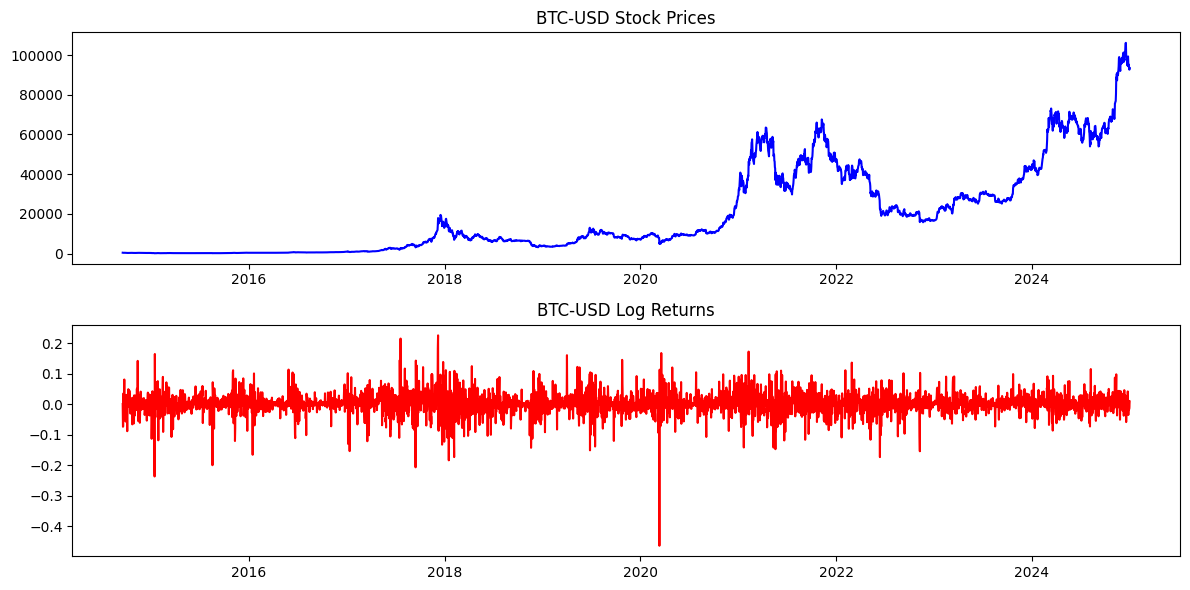
\includegraphics[width=1.00\linewidth]{img/bitcoin_prices.png}
        %\caption{Enter Caption}
    \end{figure}
    At first glance, the sharp decline of more than 40$\%$ in the BTC-USD price on March 12, 2020 is evident.
    
    \item \textbf{Constrution of the lag-plot:}\\
        We now construct the lag-plot (time-delay embedding) by plotting the log-returns against their past values, obtaining:
    \begin{figure}[H]
        \centering
        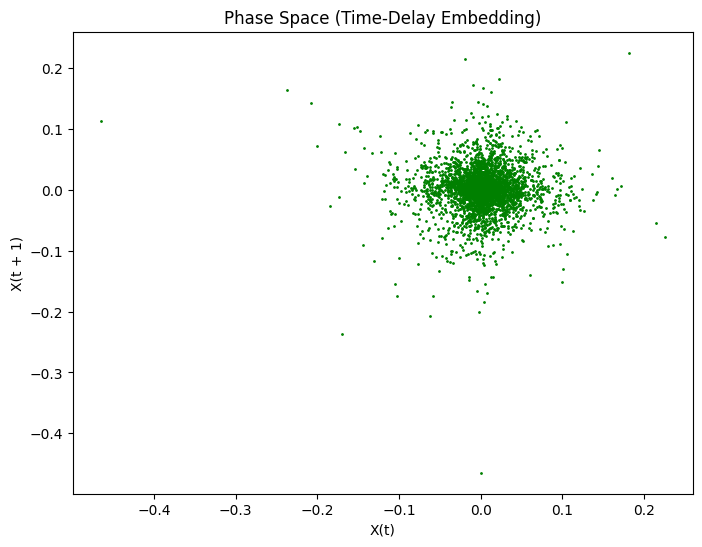
\includegraphics[width=0.75\linewidth]{img/lag_plot_bitcoin.png}
        \caption{Lag-plot of Bitcoin log-returns.}
    \end{figure}
    This plot represents a simple two-dimensional strange attractor. It shows how chaotic the stock return series behaves over time.
    
    \item \textbf{Calculation of the fractal dimension (correlation dimension):}\\
    We first compute the Euclidean distance between every pair of points in the previous lag-plot, thereby obtaining the distribution of separations between states. We then introduce a sequence of radii $\{r_i\}_i$ and for each radius value we count how many pair of points $C(r_i)$are closer than $r_i$. This produces a set of values $C(r)$ as a function of $r$, which can subsequently be represented o a log-log scale:


    \begin{figure}[H]
        \centering
        \begin{subfigure}[t]{0.49\textwidth}
            \centering
            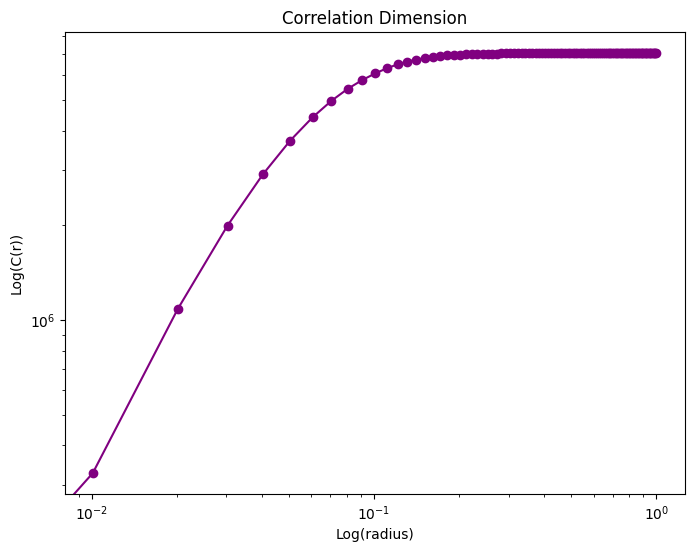
\includegraphics[width=\linewidth]{img/bitcoin_dimension.png}
            \label{fig:bitcoin_dimension}
        \end{subfigure}
        \hfill
        \begin{subfigure}[t]{0.49\textwidth}
            \centering
            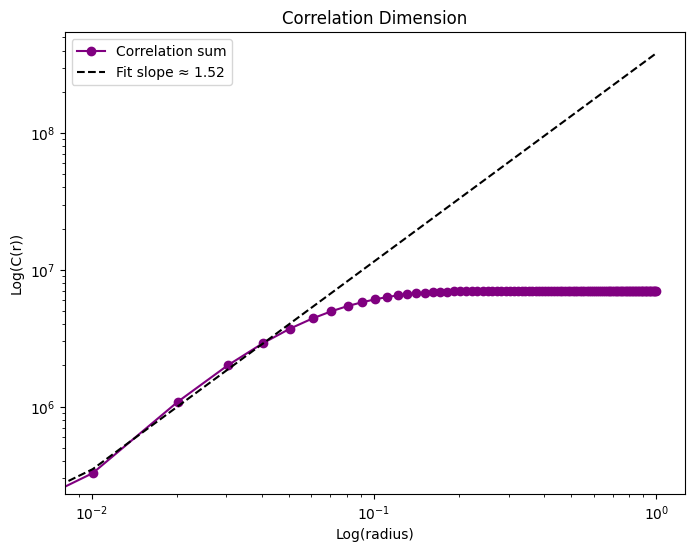
\includegraphics[width=\linewidth]{img/correlation_dimension.png}
            \label{fig:correlation_dimension}
        \end{subfigure}
        \caption{Estimation of Bitcoin’s correlation dimension.}
        \label{fig:dimension_estimation}
    \end{figure}
    
    As described in Appendix \ref{app:C_Correlation_dimension}, it is possible to estimate the correlation dimension (fractal dimension) by measuring the slope of the initial linear portion of the plot:
    
    So the estimated fractal dimension of the system is about $1.52$.
    
    A non-integer fractal dimension (such as $1.52$) is typical of chaotic attractors (strange attractors): it indicates that the system possesses a complex geometric structure, with trajectories that intertwine without ever repeating exactly.
    
    \item \textbf{BTC-USD price forecasts}\\
    Using the k-NN algorithm described in section \ref{sec:k-NN_method}, one can proceed to make BTC-USD price forecasts:
    \begin{figure} [H]
        \centering
        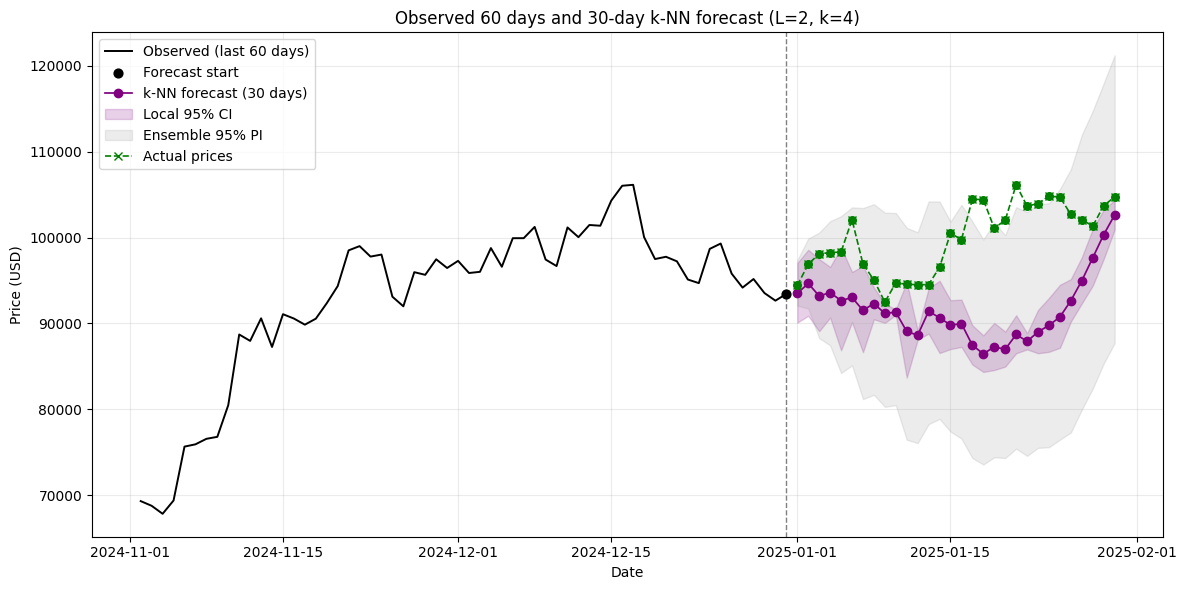
\includegraphics[width=1\linewidth]{img/forecast.png}
        \caption{Price over the last 60 days (black) and 30-day k-NN forecast (purple).}
    \end{figure}
    Here we plotted the prices for the last 60 days (black) and the 30-day ahead forecasts produced by the k-NN algorithm (in purple). The actual prices for January 2025 are shown in green.
    
   As shown in the chart, our forecasts are able to closely follow the actual prices only during the very first days. After that, they tend to reproduce merely the overall trend rather than the precise fluctuations. This outcome is not surprising, since the k-NN algorithm is inherently a one-step-ahead forecasting method. When applied iteratively, it inevitably accumulates errors at each step, which progressively amplifies the discrepancy from the true values.\\
   
   Moreover, due to its intrinsic structure—based on “local” interpolation—it can only capture short-term, local dynamics (and possibly local chaotic behavior) in the phase space. It is not designed to recognize or reproduce broader chaotic patterns, which further explains why its predictions gradually diverge from the actual price trajectory.\\
   
    \textit{(Some may view this as empirical evidence supporting the Efficient Market Hypothesis (EMH), but remember that we used a very simplistic algorithm, and far more complex and accurate methods exist that also make use of machine learning.)}
\end{itemize}

\newpage

\appendix

\section{Asymptotic Normality of the Random Walk} \label{app:A}
In this appendix we provide a concise demonstration of why the distribution of a \textit{simple random walk} converges to the \textit{normal} law as the number of steps increases.\\
\begin{proof}
Consider independent random variables $X_1, X_2, \hdots$ where each variable is either $+1$ or $-1$, with a $50\%$ probability for either value.
Let 
\begin{equation*}
    S_n \equiv \sum_{j=1}^n X_j
\end{equation*}
the series $\left\{S_n\right\}$ is called \textit{simple random walk} on $\mathbb{Z}$. This series (the sum of the sequence of $-1s$ and $+1s$) gives the net distance walked, if each part of the walk is of length one. By linearity of expectation, we have 
\begin{equation*}
    \mathbb{E}[S_n]= \sum_{j=1}^n \mathbb{E}[X_j] = 0
\end{equation*}
That is, the mean of all coin flips approaches zero as the number of flips increases.
A similar calculation, using the independence of the random variables and the fact that $\mathbb{E}[X_j^2] = 1$
\begin{equation*}
    \mathbb{E}[S^2_n] = \sum_{j=1}^2 \mathbb{E}[X_j^2] + 2\sum_{1\leq i \leq j \leq n}^n \mathbb{E} [X_i X_j] = n
\end{equation*}
%This hints that $\mathbb{E}\left[\abs{S_n}\right]$, the expected translation distance after n steps, should be of the order of $\sqrt{n}$. In fact 
%\begin{equation*}
%    \lim_{n \to \infty} \frac{\mathbb{E}[\abs{S_n}]}{\sqrt{n}} = \sqrt{\frac{\pi}{2}}
%\end{equation*}
Consider $\{S_n\}$, the random walk of $n$ steps, where each step is either $+1$ or $-1$. 
There are $2^n$ possible walks in total. 

If the sum of the steps is $S_n = k$, then the number of $+1$ steps must exceed 
the number of $-1$ steps by $k$. This means that $(n+k)/2$ must be an integer, 
and exactly $(n+k)/2$ of the $n$ steps must be $+1$. 
The number of such walks is therefore
\begin{equation*}
    \binom{n}{(n+k)/2}
\end{equation*}
where it is understood that $n+k$ must be even. 
Hence, the probability that $S_n = k$ is
\begin{equation*}
    P(S_n = k) = 2^{-n} \binom{n}{(n+k)/2}
\end{equation*}

For large $n$, these probabilities can be estimated using Stirling’s approximation:
\begin{equation*}
    \ln (n!) \approx n \ln n - n + \frac{1}{2} \ln (2 \pi n) \quad \text{as } n \to \infty  
\end{equation*}
Thus, 
\begin{equation*}
    \ln P(S_n = k) 
    = n \left[ \left(1 + \frac{k}{n} \right) \ln \left(1 + \frac{k}{n} \right) 
    + \left(1 - \frac{k}{n} - \frac{1}{2n} \right) \ln \left(1 - \frac{k}{n} \right) \right] 
    + \ln \frac{\sqrt{2}}{\sqrt{\pi}} + o(1)
\end{equation*}

Fixing the scaling $k = \lfloor \sqrt{n} x \rfloor$, for $x$ fixed, and using the expansion 
\begin{equation*}
    \ln \left(1 + \frac{k}{n}\right) = \frac{k}{n} - \frac{1}{2}\left(\frac{k}{n}\right)^2 + \ldots
\end{equation*}
when $k/n$ vanishes, it follows
\begin{equation*}
    P\left( \frac{S_n}{\sqrt{n}} = \frac{\lfloor \sqrt{n}x \rfloor}{\sqrt{n}} \right) = \frac{1}{\sqrt{n}} \cdot \frac{1}{\sqrt{2\pi}} e^{-x^2/2} \, (1 + o(1))
\end{equation*}

Taking the limit (and observing that $1/\sqrt{n}$ corresponds to the spacing of the scaling grid) one finds the Gaussian density
\begin{equation*}
    f(x) = \frac{1}{\sqrt{2\pi}} e^{-x^2/2}
\end{equation*}
\end{proof}

\section{From Black–Scholes to the Heat Equation} \label{app:B}
The Black–Scholes partial differential equation can be transformed into the classical heat equation.
\begin{proof}
    Consider the Black Scholes equation (\ref{eq:Black–Scholes}); let's make the following change of variables:
    \begin{align*}
        S &= e^{x} \\
        t &= T - \frac{\tau}{\sigma^2}
    \end{align*}
    
    \begin{equation*}
        V(S,t) = v(x,\tau) = v\!\left(\ln(S), \frac{\sigma^2}{2}(T - t)\right)
    \end{equation*}

    Calculating the respective derivatives present in the original equation
    
    \begin{equation*}
        \pdv{V}{t} = \pdv{v}{\tau} \pdv{\tau}{t} 
        = -\frac{\sigma^2}{2} \pdv{v}{\tau}
    \end{equation*}
    
    \begin{equation*}
        \pdv{V}{S} = \pdv{v}{x} \pdv{x}{S} 
        =  \frac{1}{S} \pdv{v}{x}
    \end{equation*}
    
    \begin{align*}
        \pdv[2]{V}{S} &= \pdv{s} \left( \pdv{v}{S} \right) = \pdv{S} \left( \frac{1}{S} \pdv{v}{x} \right) \\
        &= -\frac{1}{S^2}\pdv{v}{x} + \frac{1}{S} \pdv{}{x} \pdv{x}{S} \pdv{v}{x} \\
        &= -\frac{1}{S^2}\pdv{v}{x} + \frac{1}{S^2} \pdv{}{x} \pdv{v}{x} \\
        &= -\frac{1}{S^2}\pdv{v}{x} + \frac{1}{S^2}\pdv[2]{v}{x}
    \end{align*}
    
    Reinserting the transformed derivatives into the Black–Scholes equation and collecting similar terms.
    
    \begin{equation*}
        \pdv{v}{\tau} = \pdv[2]{v}{x} + \left(\frac{2r}{\sigma^2} - 1 \right)\pdv{v}{x} - \frac{2r}{\sigma^2} v
    \end{equation*}

    After consolidating the parameters, we set $\kappa = \tfrac{2r}{\sigma^{2}}$ and replace $\tau$ with $t$. We also adjust the domain accordingly.
    
    \begin{equation*}
        \pdv{v}{t} 
        = \pdv[2]{v}{x} 
        + (\kappa - 1)\pdv{v}{x} 
        - \kappa v
    \end{equation*}
    
    The new equation is similar to the heat equation, except for two terms on the right-hand side, which we eliminate through another change of variables.
    
    \begin{equation*}
        v(x,t) = e^{\alpha x + \beta t}(x,t) = \psi u
    \end{equation*}
    
    Let us recompute the derivatives of the given expressions:
    
    \begin{equation*}
        \pdv{v}{t} = \beta \psi u + \psi \pdv{u}{t}
    \end{equation*}

    \begin{equation*}
        \pdv{v}{x} = \alpha \psi u + \psi \pdv{u}{x}
    \end{equation*}
    
    \begin{align*}
        \pdv[2]{v}{x} &= \pdv{}{x} \left( \alpha \psi u + \psi \pdv{u}{x} \right) \\
         &= \alpha^2 \psi u + 2 \alpha \psi \pdv{u}{x} + \psi \pdv[2]{u}{x}
    \end{align*}

    By inserting the derivatives into the transformed PDE, we rearrange the expression, collect like terms, and cancel the factor $e^{\alpha x + \beta t}$, which, being exponential, is always positive.

    \begin{equation*}
        \pdv{u}{t} = \pdv[2]{u}{x} + \left[ 2\alpha + (k - 1) \right] \pdv{u}{x} + \left[ \alpha^2 + (k - 1)\alpha - k - \beta \right] u
    \end{equation*}

    As $\alpha$ and $\beta$ are arbitrary, we select them to remove both the $\pdv{u}{x}$ and $u$ contributions.

    \begin{align*}
        \alpha &= \frac{k - 1}{2} \\
        \beta  &= \alpha^2 + (k - 1)\alpha - k = -\frac{(k + 1)^2}{4}
    \end{align*}

    At this stage, the equation reduces to the one-dimensional heat equation.

    \begin{equation*}
        \pdv{u}{t} = \pdv[2]{u}{x}
    \end{equation*}


    \subsection{Derivation of the Solution}\label{app:B_solution_Black-Scholes}
    At this point, the standard representation formula for solutions of the heat equation can be used in the context of the Black--Scholes equation.
    \begin{equation*}
        u(x,\tau) = \frac{1}{2\sqrt{\pi \tau}} \int_{-\infty}^{+\infty} u_0(s) \exp\!\left(-\frac{(x - s)^2}{4\tau}\right) \, \dd{s}
    \end{equation*}
    We perform the following change of variable
    \begin{equation*}
        z = \frac{s - x}{\sqrt{2\tau}} \qquad \Longrightarrow \qquad \dd{z} = - \frac{1}{\sqrt{2\tau}}\,\dd{x}
    \end{equation*}
    \begin{equation*}
        u(x,\tau) = \frac{1}{2\sqrt{\pi}} \int_{-\infty}^{+\infty} u_0\left(z\sqrt{2\tau+x}\right)\, \exp({-z^2/2})\,\dd{z}
    \end{equation*}

    \begin{equation*}
        u_0 = e^{-\tfrac{k-1}{2}}\,(e^x - 1) = e^{\tfrac{k+1}{2}\,\left(x + z\sqrt{2\tau}\right)} - e^{\tfrac{k-1}{2}\,\left(x + z\sqrt{2\tau}\right)}
    \end{equation*}
    
    We consider two separate integrals:
    \begin{align*}
        I_1 &= \frac{1}{2\sqrt{\pi}} \int_{-\tfrac{x}{2\tau}}^{+\infty} e^{\tfrac{k+1}{2}\,\left(x + z\sqrt{2\tau}\right)} \, e^{-z^2/2}\dd{z} \\
        I_2 &= \frac{1}{2\sqrt{\pi}} \int_{-\tfrac{x}{2\tau}}^{+\infty} e^{\tfrac{k-1}{2}\,\left(x + z\sqrt{2\tau}\right)} \, e^{-z^2/2}\dd{z}
    \end{align*}
    
    After an algebraic manipulation of the exponent, we obtain
    \begin{equation*}
        \frac{e^{\tfrac{(k+1)^2 \tau}{4}} + e^{\tfrac{(k+1)x}{2}}}{\sqrt{2\pi}} \int_{-\tfrac{x}{2\tau}}^{+\infty} \exp(-\tfrac{1}{2}\left(z - (k+1)\sqrt{\tau / 2}\right)^2) \dd{z}
    \end{equation*}

    Following another change of variable
    \begin{equation*}
        y = z - \sqrt{\tau / 2}\,(k+1) 
        \qquad \Longrightarrow \qquad 
        \dd{y} = \dd{z}
    \end{equation*}

    \begin{equation*}
       \frac{e^{\tfrac{(k+1)^2 \tau}{4}} + e^{\tfrac{(k+1)x}{2}}}{\sqrt{2\pi}} \int_{-x/(2\tau) - \sqrt{\tau / 2} (k+1)}^{+\infty} e^{-y^2/2}\,\dd{y}
    \end{equation*}
    
    The integral represents the cumulative distribution function $\phi$ of a normal variable $d$.
    \begin{equation*}
        \phi(d) = \frac{1}{\sqrt{2\pi}} \int_{-\infty}^{d} e^{-y^2/2} \dd{y}
    \end{equation*}
    Thus
    \begin{equation*}
        I_1 = \left[e^{\tfrac{(k+1)^2 \tau}{4}} + e^{\tfrac{(k+1)x}{2}}\right] \, \phi(d_1),
        \qquad 
        d_1 = \frac{x}{2\tau} + \sqrt{\tau / 2}\,(k+1)
    \end{equation*}
    
    To obtain $I_2$ one proceeds as before but replaces $(k+1)$ with $(k-1)$.
    \begin{equation*}
        u(x,\tau) = \left[ e^{\tfrac{(k+1)^2 \tau}{4}} + e^{\tfrac{(k+1)x}{2}}\right] \, \phi(d_1) - \left[e^{\tfrac{(k-1)^2 \tau}{4}} + e^{\tfrac{(k-1)x}{2}}\right] \, \phi(d_2)
    \end{equation*}
    
    We must undo the changes of variables, obtaining
    \begin{equation*}
        V(S,t) = S\,\phi(d_1) - e^{-r(T-t)}\,\phi(d_2)
    \end{equation*}
    where
    \begin{align*}
        d_1 &= \frac{\ln(S) + \left(r + \sigma^2 / 2 \right)(T - t)}{\sigma \sqrt{T - t}} \\
        d_2 &= \frac{\ln(S) + \left(r - \sigma^2 / 2\right)(T - t)}{\sigma \sqrt{T - t}}
    \end{align*}

\end{proof}

\section{Measures of Fractal dimension} \label{app:C}
The traditional Euclidean notion of dimension cannot adequately describe the complexity and self-similar structure of fractal sets. It becomes necessary to introduce a generalized concept of dimension that extends beyond the integer-valued dimension in classical geometry.\\

The idea becomes clearer when we consider the von Koch curve. Being a curve, its Euclidean dimension is 1 (geometrically one-dimensional). However, due to its fractal nature, the distance along the curve between any two points is infinite.
This highlights the need for a concept of dimension that takes into accounts the fact that the curve occupies "more space" than an ordinary curve, but "less space" than a surface.
\begin{figure}[H]
        \centering
        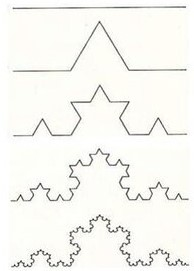
\includegraphics[width=0.35\linewidth]{img/curva di Van Koch.jpg}
        \caption{Creation of the Von Koch curve.}
        %\label{fig:placeholder}
\end{figure}

\subsection{Box-dimension} \label{app:C_Box_dimension}
For this reason is introduced the concept of \textit{box-dimension}. How to obtain the box dimension:
\begin{enumerate}[label=\roman*)]
    \item Cover the whole set with $\varepsilon$-sized boxes (for a set of Euclidean dimension $D$, the covering boxes are $D$-dimensional cubes).
    \item Count the boxes' number $N(\varepsilon)$.
    \item Study the variation of $N(\varepsilon)$ while decreasing $\varepsilon$.
    \item Calculate the Box-dimention.
\begin{equation*}
    d=\lim_{\varepsilon \rightarrow 0} \frac{\ln(N(\varepsilon))}{\ln(1/\varepsilon)}    
\end{equation*}

\end{enumerate}

To simplify, one can say that if $N(\varepsilon)$ scales as $1/\varepsilon^d$ (for a line, $N(\varepsilon) \sim L/\varepsilon$; for a surface, $N(\varepsilon) \sim~A/\varepsilon^2$), then $d$ is the box dimension of the set. This is the case for "well-behaved" fractal sets, such as the Cantor set or the von Koch curve.


\subsection{Correlation dimension} \label{app:C_Correlation_dimension}
When analyzing chaotic systems, the correlation dimension is employed as a measure of fractal dimension, particularly in cases where one works with a set of random points (as in the case study of paragraph \ref{sec:Chaos_BTC}).\\

Compared to the box-counting dimension, the correlation dimension offers several advantages: it can be computed more easily and efficiently, it is less sensitive to noise when only a limited number of points are available, and it often yields results consistent with other dimension estimates (as box-dimension).\\

For any set of $N$ points in a $m$-dimensional space:
\begin{equation*}
    \vb{x}(i)=[x_1(i),\dots,x_m(i)], \quad i=1,2,\dots,N
\end{equation*}
the correlation integral $C(\varepsilon)$ is calculated by:
\begin{equation*}
    C(r)=\lim_{N \to +\infty} \frac{g}{N^2}
\end{equation*}
where $g$ is the number of pairs of points which have a distance between them that is less than distance $r$.\\
As the number of points tends to infinity and the distance between them tends to zero, the correlaton integral, for small values of $r$ will take the form 
\begin{equation*}
    C(r) \sim r^\nu
\end{equation*}
where $\nu$ is our correlation dimension.\\
If we have enough points, a log-log graph of the correlation integral vs $r$ will yield an estimate of $\nu$.

\newpage
\nocite{*}
\printbibliography

\end{document}